\documentclass[12pt,a4paper]{article}
\usepackage[utf8]{inputenc}
\usepackage{amsmath}
\usepackage{amsfonts}
\usepackage{amssymb}
\usepackage{graphicx}
\usepackage{float}
\usepackage[font=small,labelfont=bf]{caption}
\usepackage{tabularx}
\usepackage{siunitx}
\usepackage[LGRgreek]{mathastext}
\usepackage{cancel}
\usepackage{ulem}
\usepackage{comment}

\usepackage{listings}
\usepackage{xcolor}

\definecolor{codegreen}{rgb}{0,0.6,0}
\definecolor{codegray}{rgb}{0.5,0.5,0.5}
\definecolor{codepurple}{rgb}{0.58,0,0.82}
\definecolor{backcolour}{rgb}{0.95,0.95,0.92}

\lstdefinestyle{mystyle}{
    backgroundcolor=\color{backcolour},   
    commentstyle=\color{codegreen},
    keywordstyle=\color{magenta},
    numberstyle=\tiny\color{codegray},
    stringstyle=\color{codepurple},
    basicstyle=\ttfamily\footnotesize,
    breakatwhitespace=false,         
    breaklines=true,                 
    captionpos=b,                    
    keepspaces=true,                 
    numbers=left,                    
    numbersep=5pt,                  
    showspaces=false,                
    showstringspaces=false,
    showtabs=false,                  
    tabsize=2
}

\lstset{style=mystyle}



\newcommand{\stkout}[1]{\ifmmode\text{\sout{\ensuremath{#1}}}\else\sout{#1}\fi}
%police et mise en page (marges) du document
\usepackage[T1]{fontenc}
\usepackage[top=2cm, bottom=2cm, left=2cm, right=2cm]{geometry}




\begin{document}


%-------debut titre
\begin{titlepage}
\begin{minipage}[c]{.46\linewidth}
     \begin{center}
         %-------------------LOGO--------------------
         % \includegraphics[scale=0.2]{../../../../csm_doc-commun-logo_FST_couleur_5ed57558dd.png}  
         
         \end{center}
   \end{minipage} \hfill
   \begin{minipage}[c]{.46\linewidth}
    \begin{center}
    	%-------------------LOGO--------------------
       % \includegraphics[scale=0.38]{../../../../tele.jpg}   
        \end{center}
 \end{minipage}
\newcommand{\HRule}{\rule{\linewidth}{0.5mm}}
\center
\textsc{\LARGE
Nom de la matiere
} \\[4cm]

\HRule \\[0.4cm]
{ \huge \bfseries Rapport de stage\\ [0.15cm] }
\HRule \\[15cm]
%---------------------image illustration----------------
%\includegraphics[scale=1]{image/big.png} \\ [2cm]


\begin{flushleft}
PARASSOURAMIN Alexandre\\
Master 1 Énergie \\
35003702
\end{flushleft}


\end{titlepage}
%-----Fin titre
\newpage
\thispagestyle{empty}
~


\newpage







\thispagestyle{empty}
\renewcommand{\contentsname}{Sommaire}
\tableofcontents
\newpage

\newpage
\thispagestyle{empty}
~
\newpage

\begin{flushleft}
\sf
\section*{Introduction}
\addcontentsline{toc}{section}{\protect\numberline{}Introduction}%
\setcounter{page}{1}

Dans le cadre de mon Master1 j'ai du réaliser un stage de huit semaines, le stage s'est dérouler au sein du laboratoire LE2P de l'université de la Réunion.\\

Le stage avait pour objectif le montage d'un pyranomètre à arc d'ombrage cm121, l'élaboration d'un calendrier de maintenance pour le cm121, la mise en place d'un protocole pemrettant de régler la position Nord-sud du cm121, le dévelloppement de programme sous python permettant l'analyse statistique des mesures de DHI, mais aussi d'éffectuer une étude montrant si les mesures du cm121 sont plus proche du spn1 que du tracker et finnalement de savoir  quel dispositif ont les resiltats les plus proche du tracker entre le cm121 et le spn1.
 

\section{}
 
\section{LES TRAVAUX EFFECTUÉS ET LES APPORTS DU STAGE}



\section{Montage du CM121C}

Le CM121C comporte cinq partie, la base, le pilier, la barre transversale, la barre coulissante et le support pour pyranomètre. Le montage consiste juste a assembler chaque partie à l'aide des boulons fournis.

\begin{figure}[H]
\centering
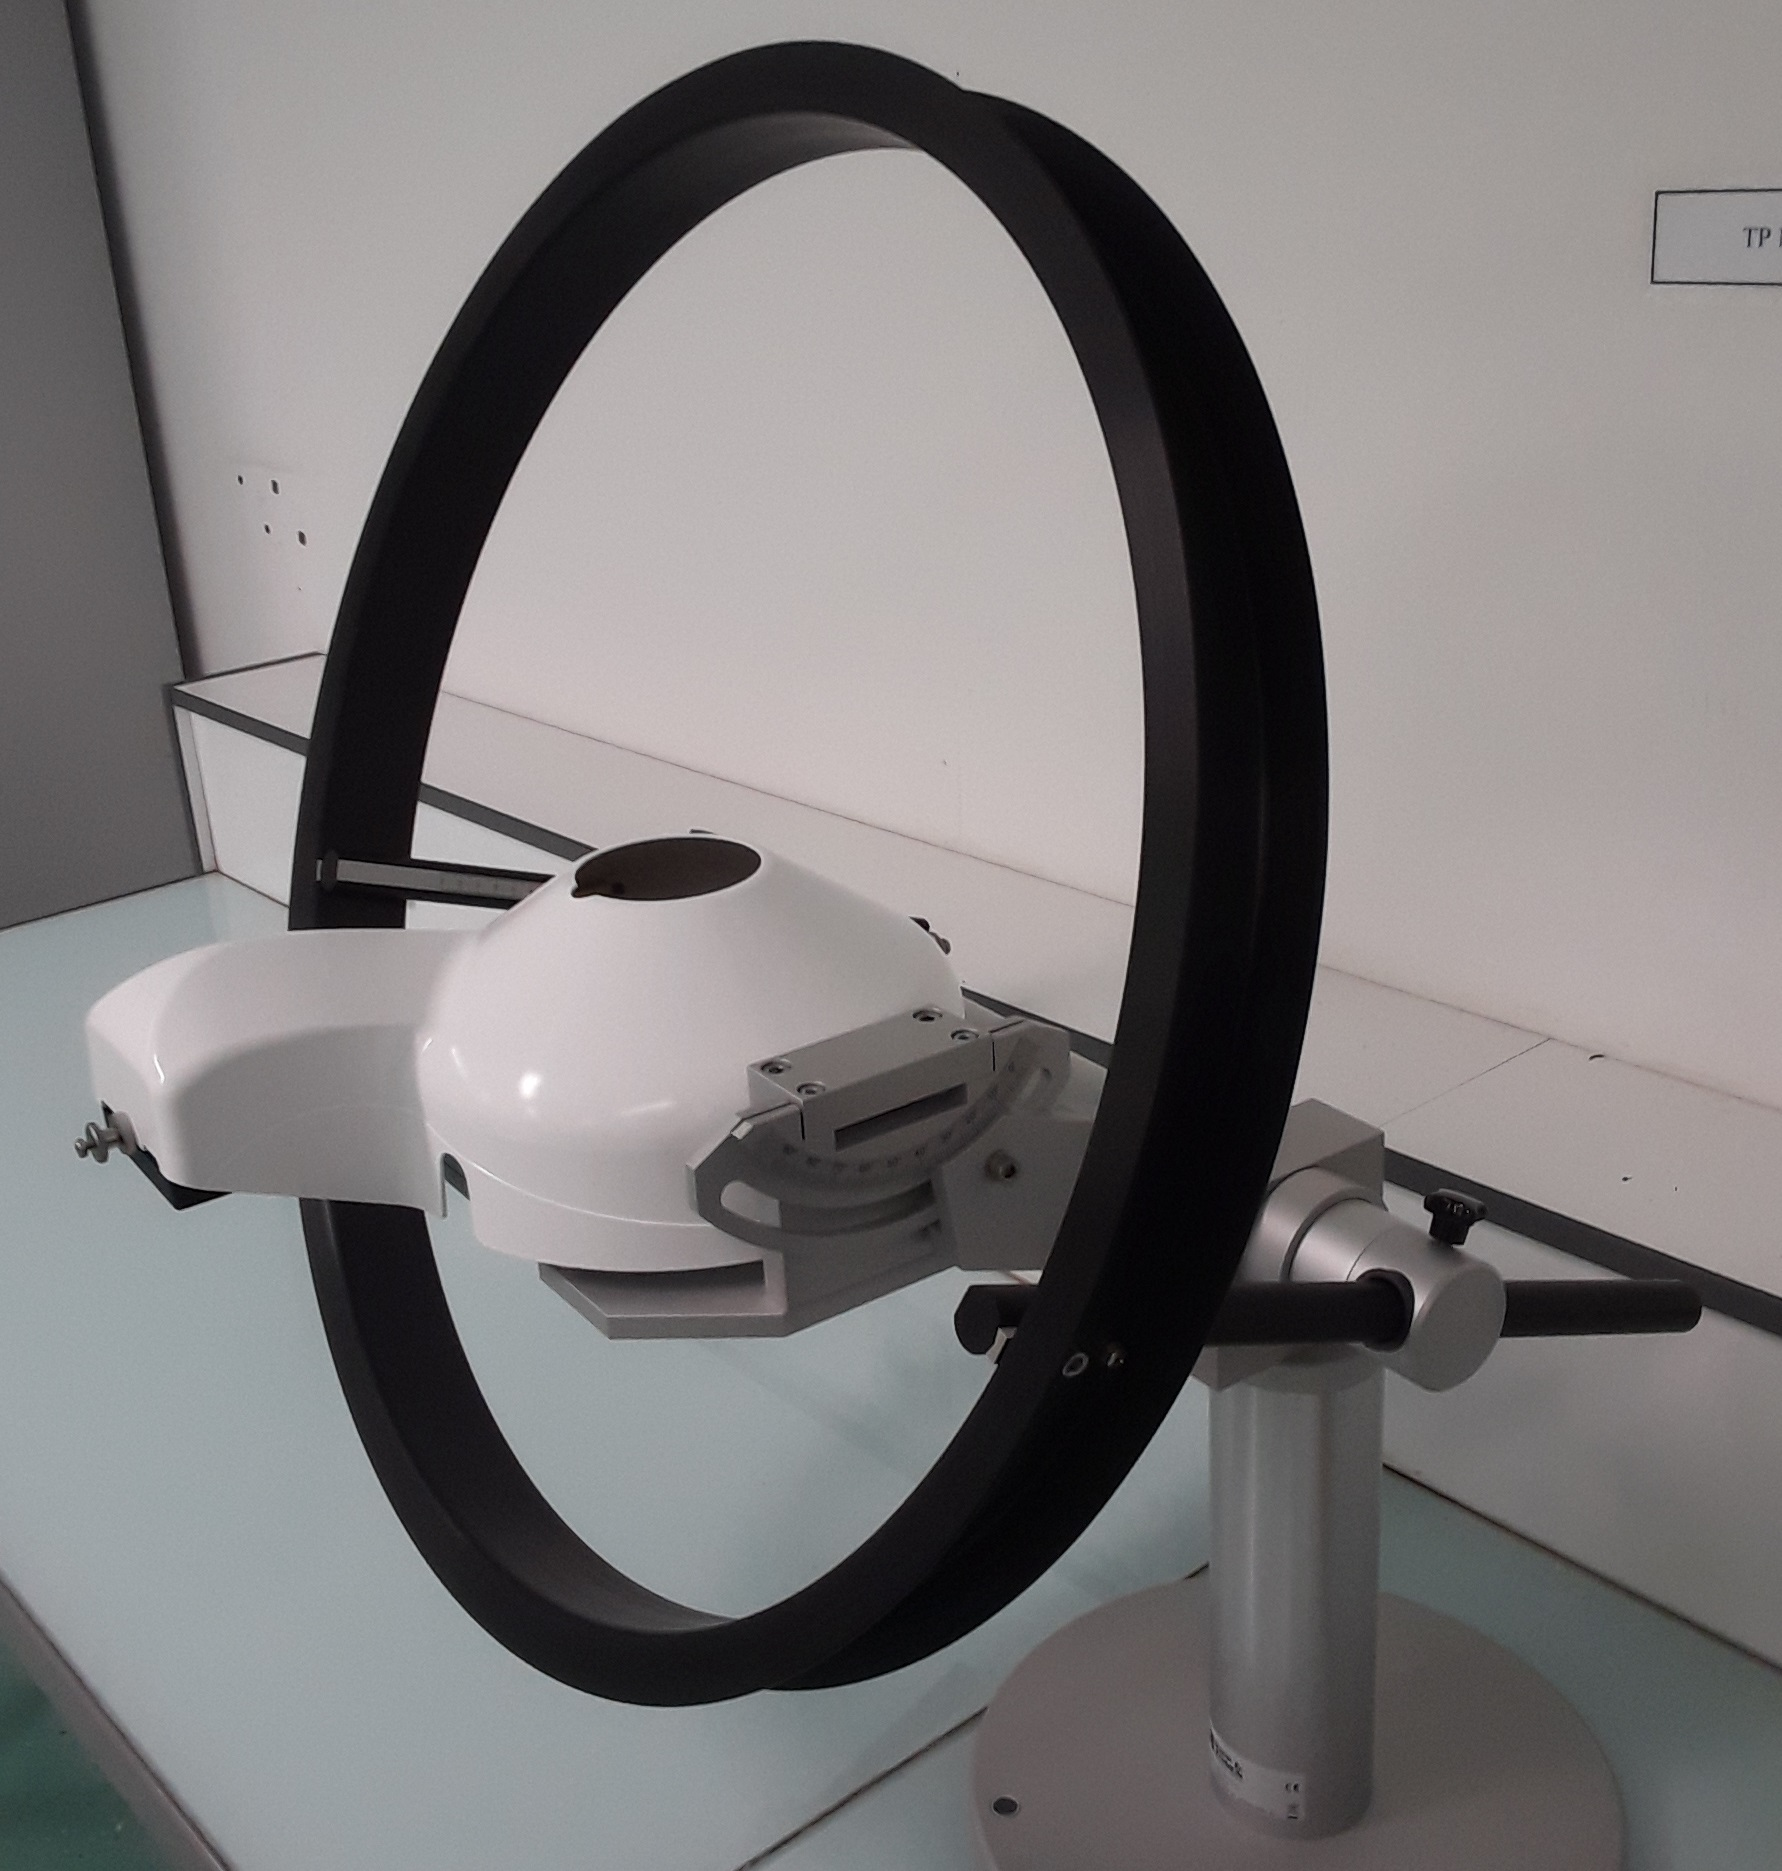
\includegraphics[width=10cm]{image/montage/1.jpg} 
\caption{cm121}
\end{figure}

\subsection{Surface Horizontal}

La premiere étape pour le positionnement du cm121 consiste à s'assurer que la base du cm121 est plane, pour se faire la base comporte 3 boulons permettant à l'aide d'un niveau à bulle de mettre la base à l'horizontal. 

\begin{figure}[H]
\centering
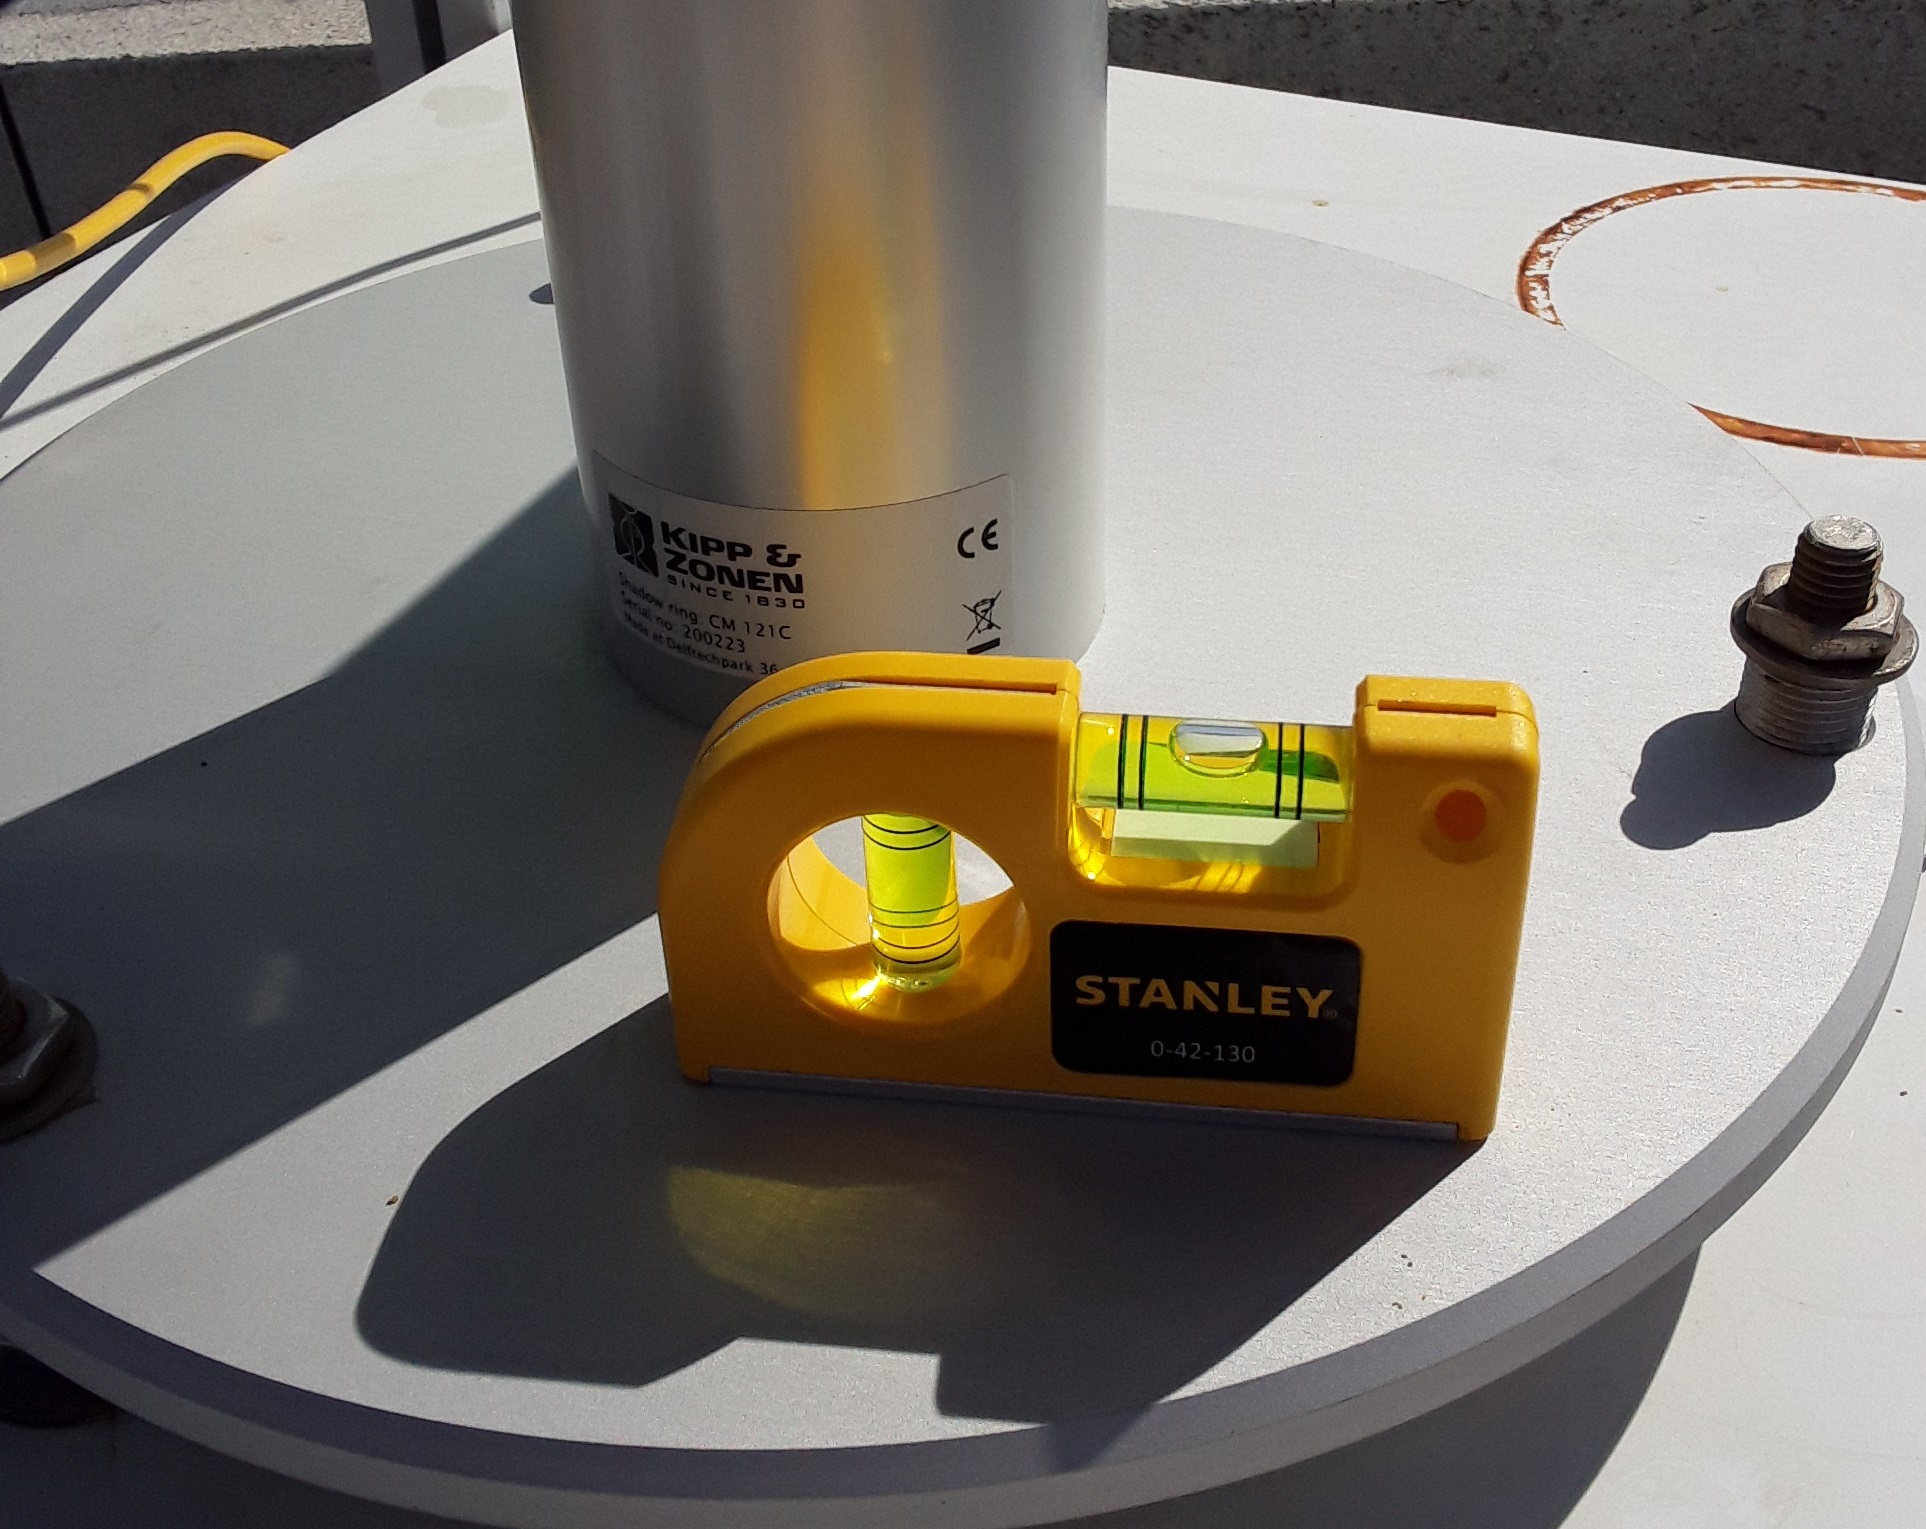
\includegraphics[width=10cm]{image/montage/2.jpg} 
\caption{Base horizontal}
\end{figure}

\subsection{Inclinaison de la barre coulissante}

La barre coullissante doit être parallele à l'axe polaire, pour se faire l'angle entre l'horizon et la barre doit etre égal à la latitude du site, pour l'Université de la réunion cela implique un angle de -20.9$^\circ$. L'angle est régler grace à une application mobile qui offre une precision suffisante le réglage pouvant se faire à 1-4 degrés prêt selon la datasheet.

\begin{figure}[H]
\centering
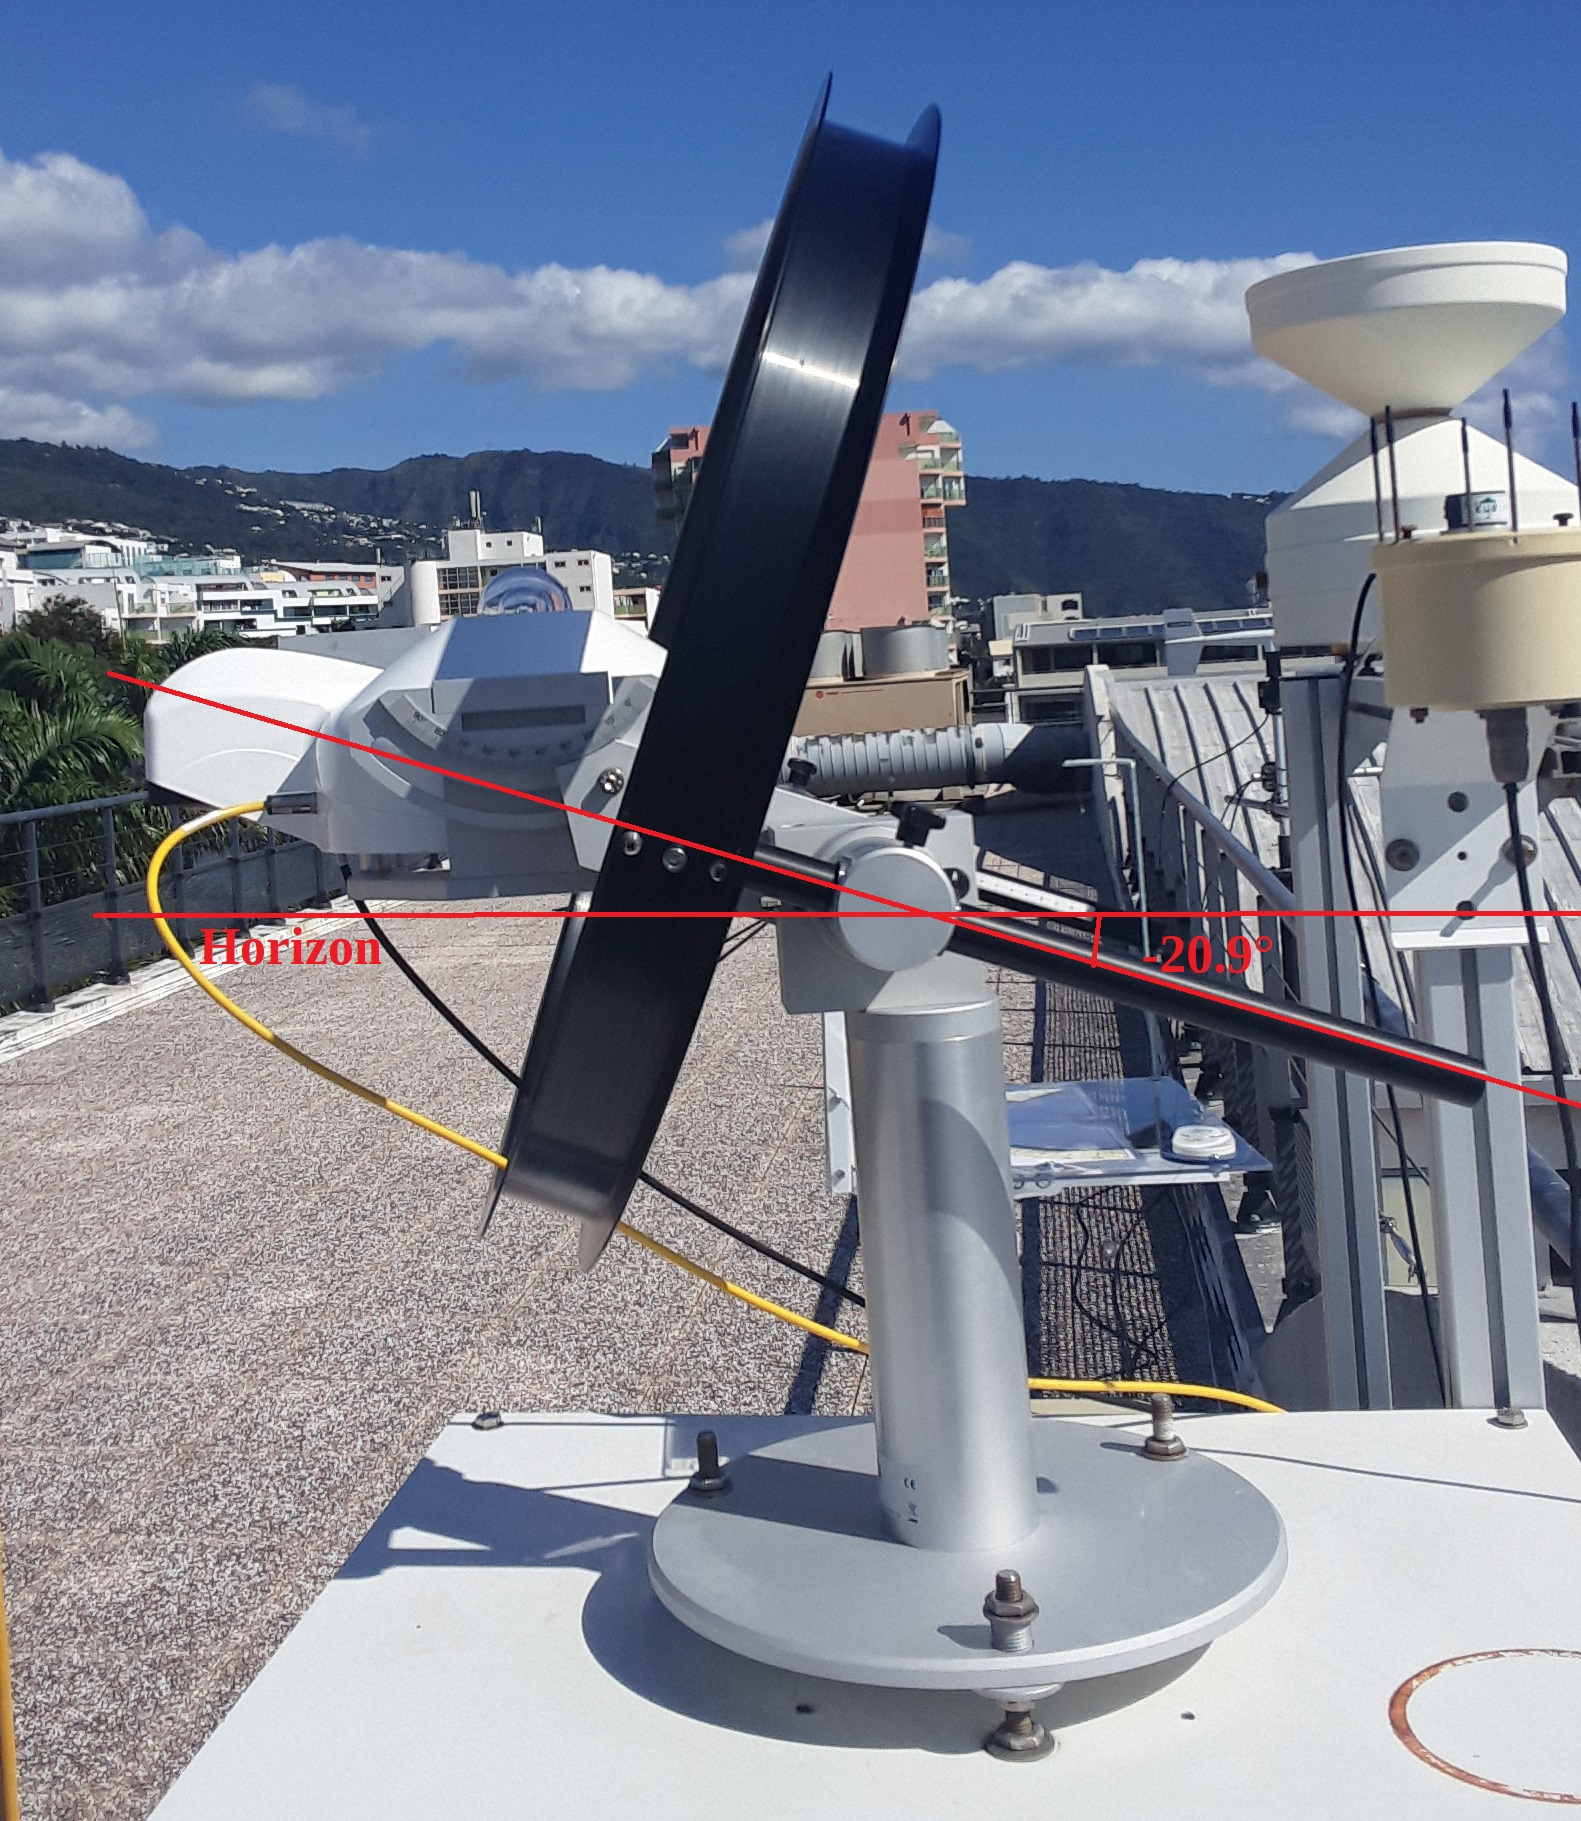
\includegraphics[width=10cm]{image/montage/3.jpg} 
\caption{Axe polaire}
\end{figure}

\subsection{Installation du pyranomètre}

Le pyranomètre est installé sur le socle prévu à cet effet, les pattes du pyranometre permettent de rattraper les erreurs d'angles lors du montage de la base. Une fois effectué la ventillation est installé est raccorder en 12 volts. La ventillation permet de garder le pyranomètre à température constante, permettant ainsi de faire l'aquisition des mesures dans les memes conditions de température toute l'année.

\begin{figure}[H]
\centering
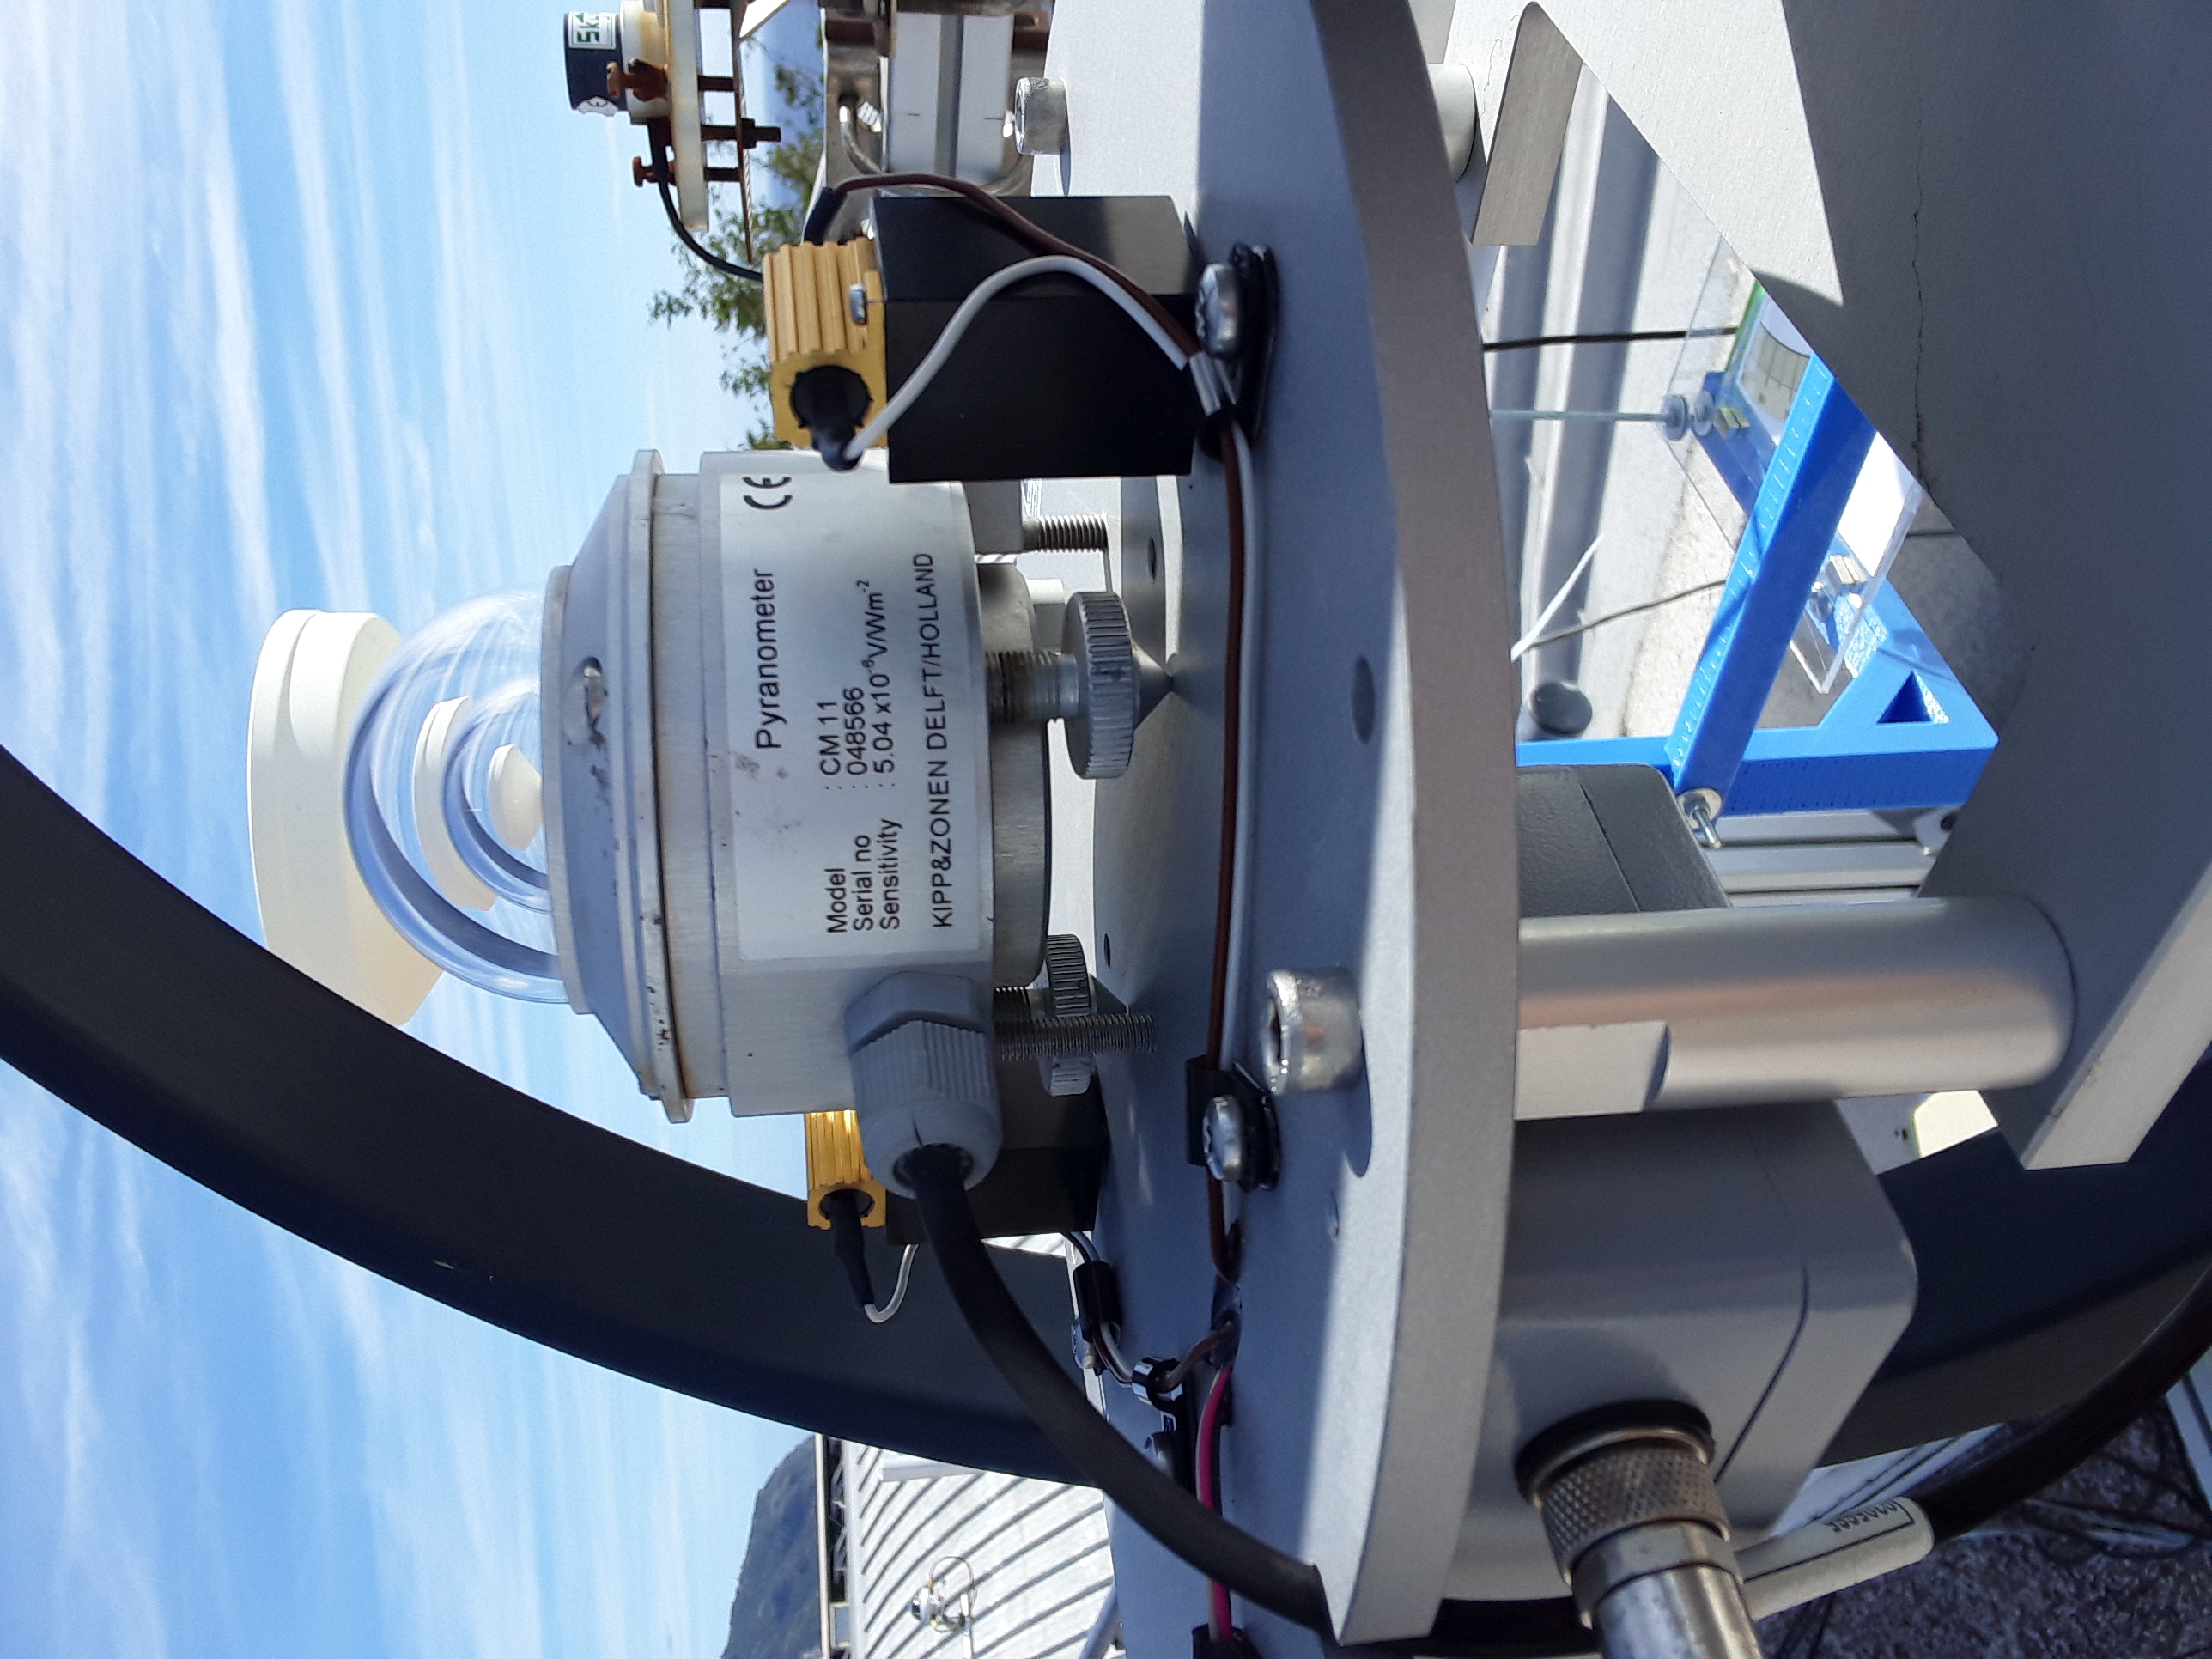
\includegraphics[width=10cm, angle=-90]{image/montage/4.jpg} 
\caption{Installation pyranomètre}
\end{figure}

\subsection{Alignement nord-sud}

L'étape la plus importante et le réglage de la position nord-sud, un mauvais reglage nord-sud peut entrainer des donnes eronné du fait que le capteur est susceptible de capter du rayonnment globale à certain moment de la journée. Une premiere approche pourrait consister à utiliser un compas magnétique mais la présence d'élément ferreux donne une indication éronné du nord. La méthode retenue est l'utilisation d'une boussole solaire.\\
~~\\
Le principe de la boussole solaire est de projeter l'ombre du soleil sur une surface plane, sur cette surface plane se trouve un cadran graduer représentant l'azimut, en connaissant l'azimut du soleil et en reportant l'ombre sur le cadran nous obtenons la positions nord-sud.\\

\subsubsection{Pointage géographique}

Le premier alignement Nord-sud fut effectué par une boussole solaire totalement independante de l'arc d'ombrage, le but consiste à l'aide d'une feuille excel et de l'heure actuel, de calculé l'azimut, de le reporté sur la boussole solaire en la faisant pivoter et de pointer un point geographique le plus lointain passant dans l'axe nord-sud de la boussole solaire. Une fois ce point geographique trouvé, nous effectuons la meme demarche en reportant ce point dans l'axe de la barrre coulissante.\\

Cette methode donne de bon résultat, mais elle nous expose à des erreurs d'angle nottament lors du pointage du point géographique et le vent faisant bouger le fil, elle a aussi pour inconvénient une mise en place assez lourde avec l'obligation d'avoir un ordinateur portable sous la main.\\	

\begin{figure}[H]
\centering
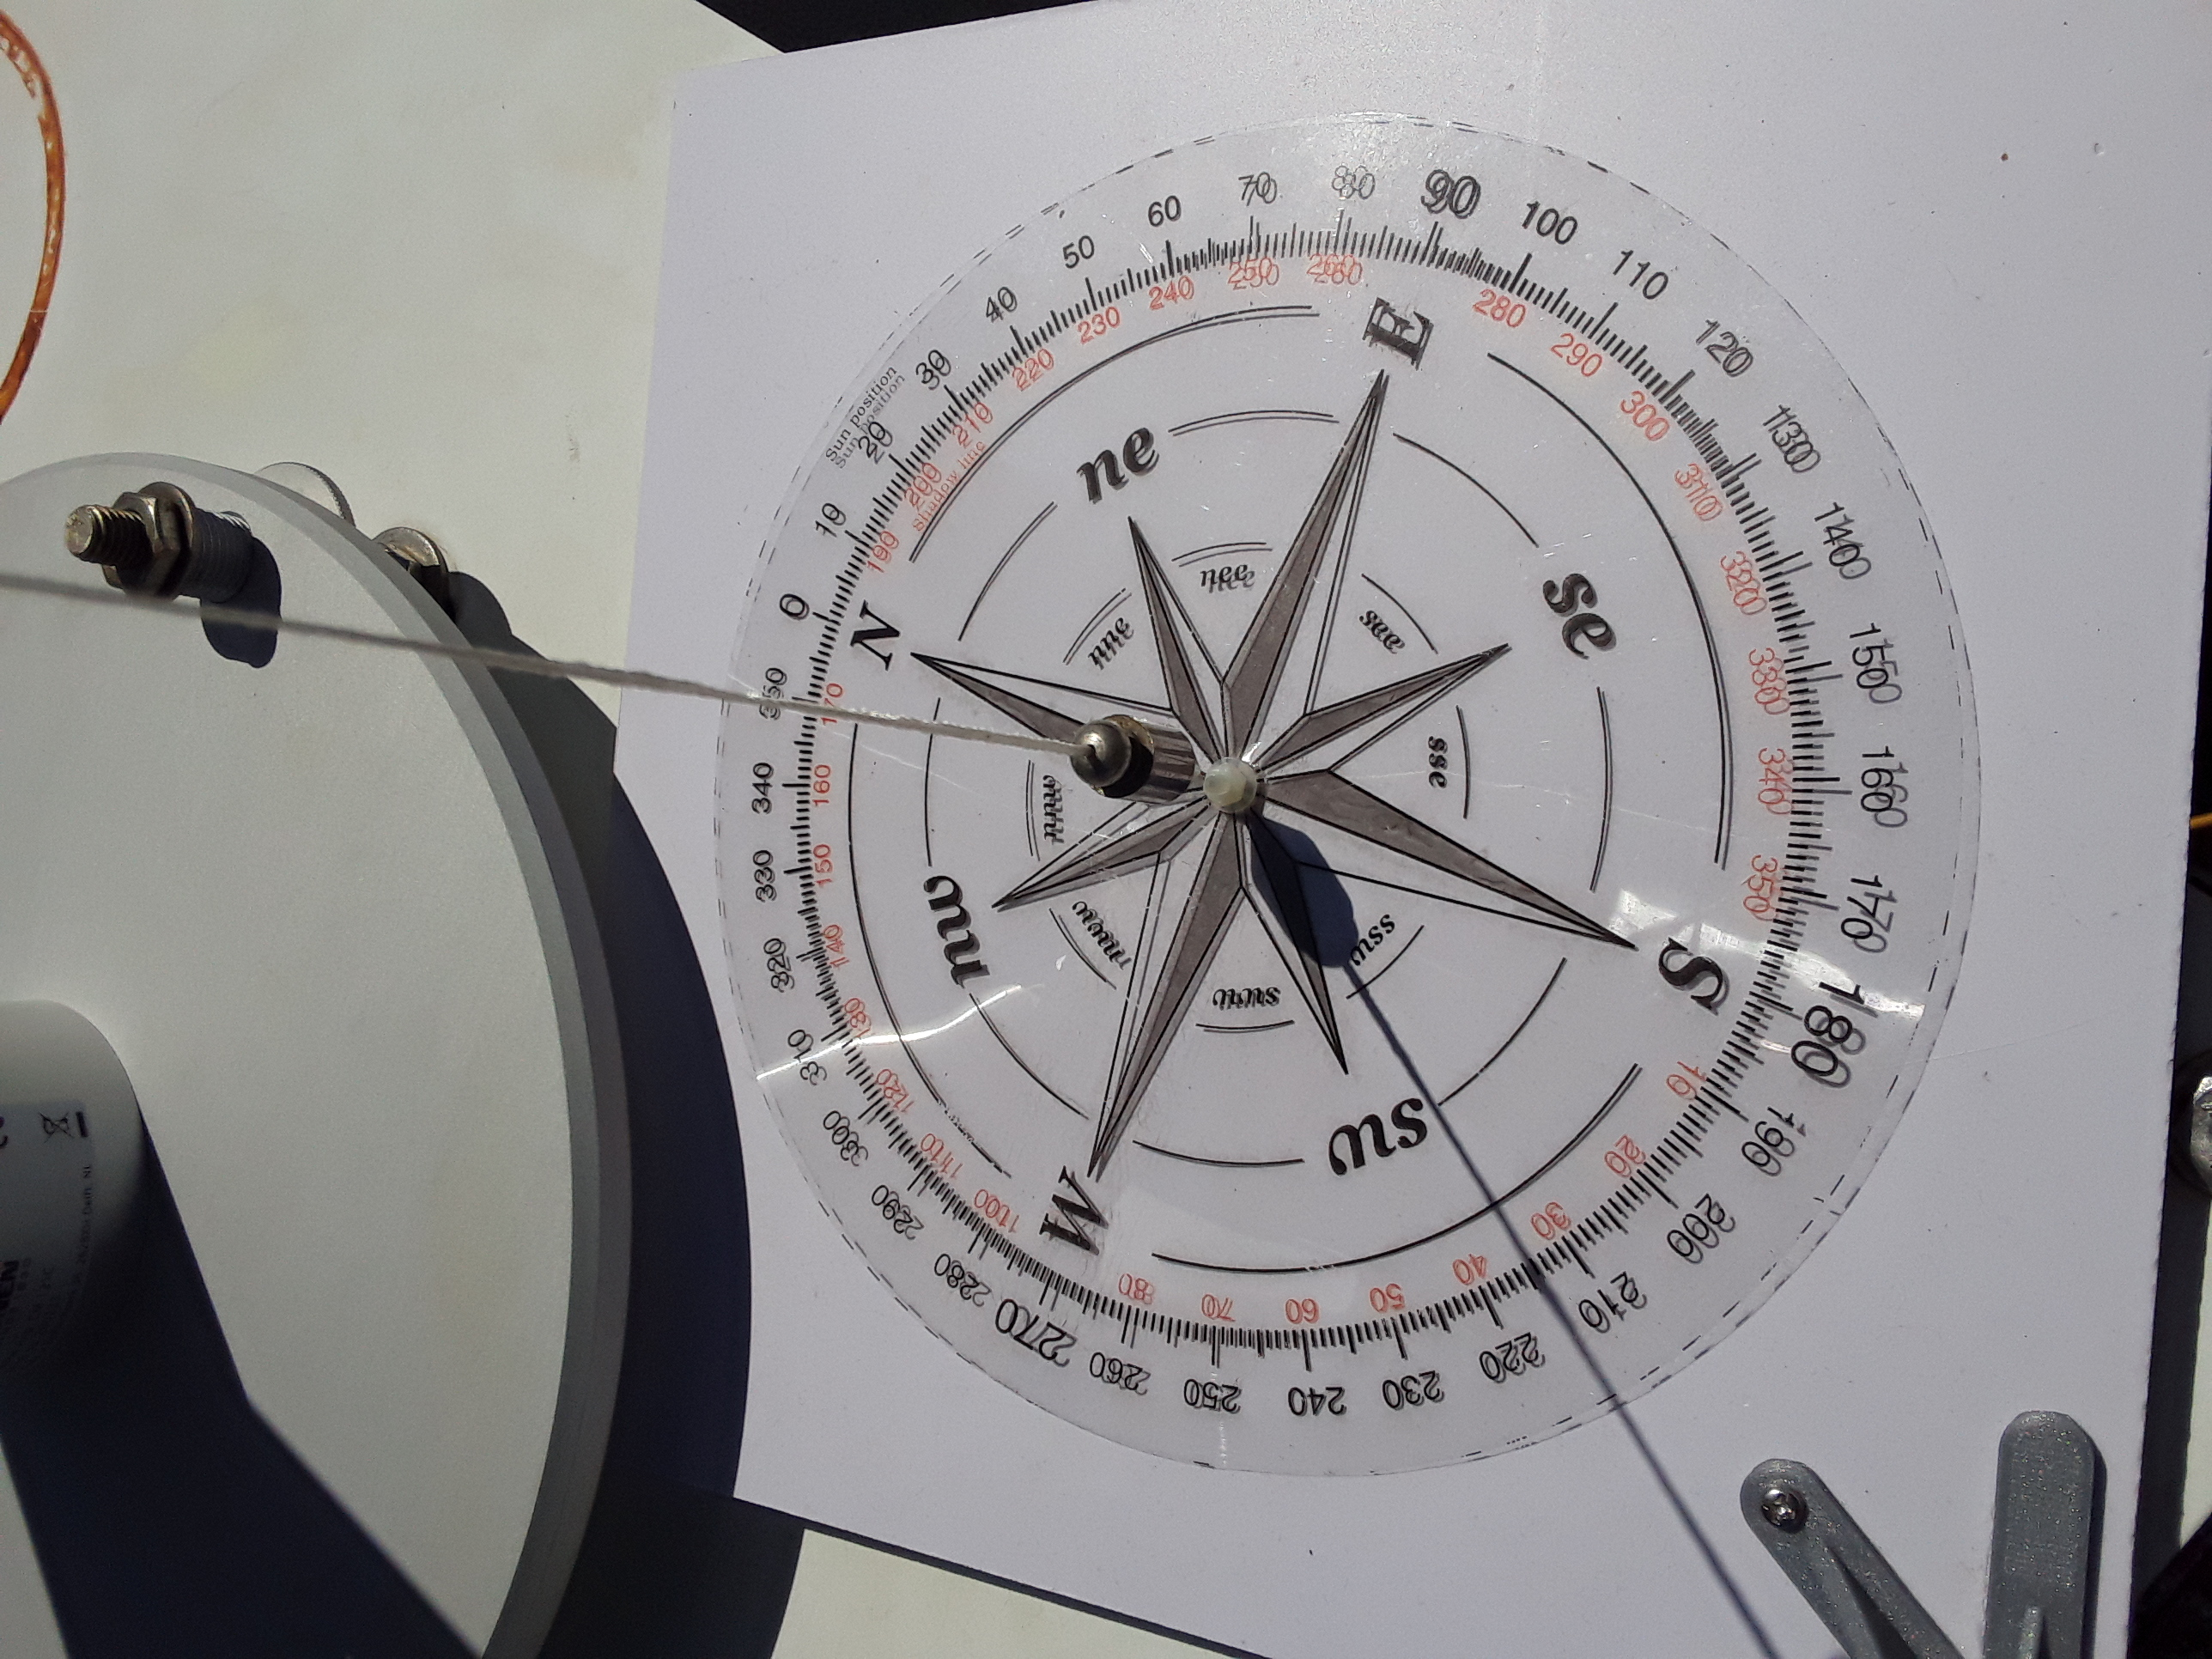
\includegraphics[width=10cm, angle=-90]{image/montage/5.jpg} 
\caption{Boussole solaire}
\end{figure}

\begin{figure}[H]
\centering
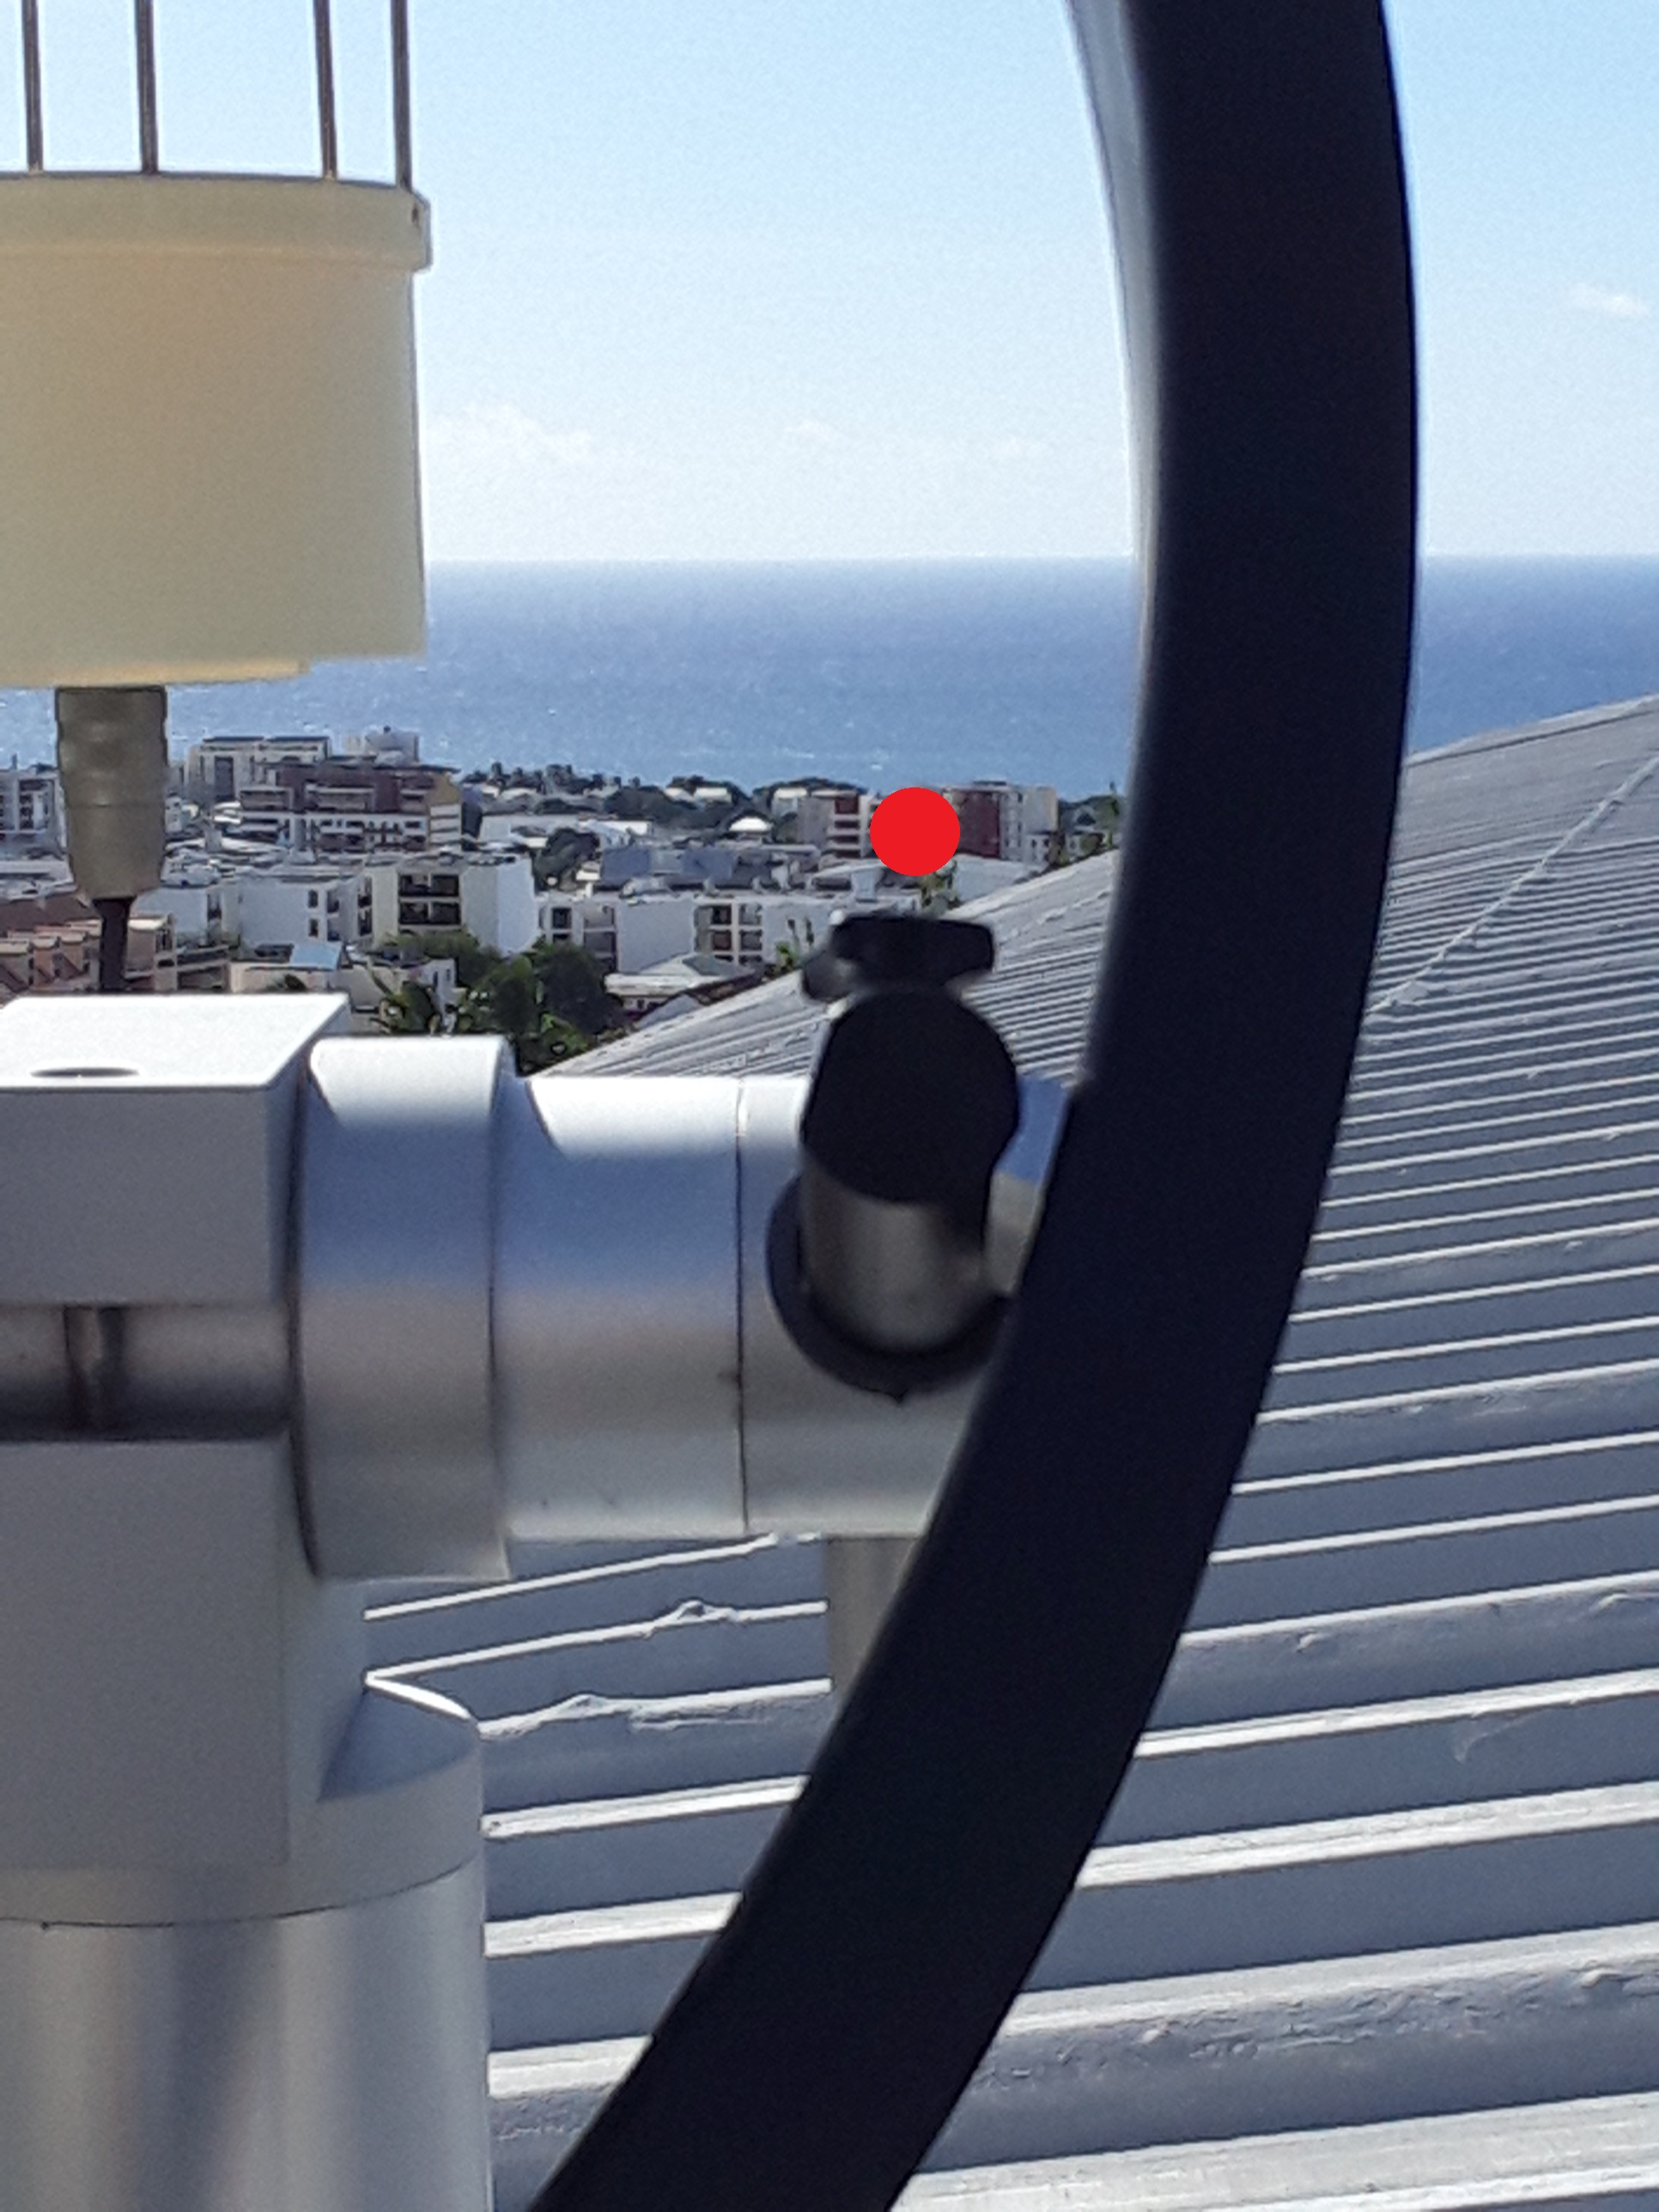
\includegraphics[width=10cm]{image/montage/6.jpg} 
\caption{Point géographique}
\end{figure}

\subsubsection{Boussole solaire fixe}   

Pour palier aux problèmes de la boussole solaire traditionnelle, il fut elaborer une boussole solaire fixe. Le but est de faciliter le réglage nord-sud, mais aussi de diminuer les erreurs d'angles de la boussole traditionnelle, pour se faire la boussole devras etre fixer à la barre transversale du cm121.\\
~\\
Pour faciliter la maintenance le choix de la conception c'est porté sur l'impression 3D et la modélisation fut effectué sur le logiciel fusion 360 (figure *). La boussole comporte 4 partie imprimer en 3D (deux bases et deux longerons), une plaque de plexiglas permettant de placer notre cadran d'azimut et une tige filleté qui sert de support au fil.\\



Les quatre parties imprimé en 3D sont assembler à l'aide de quatre boulon de 3*20mm.\\

\begin{figure}[H]
\centering
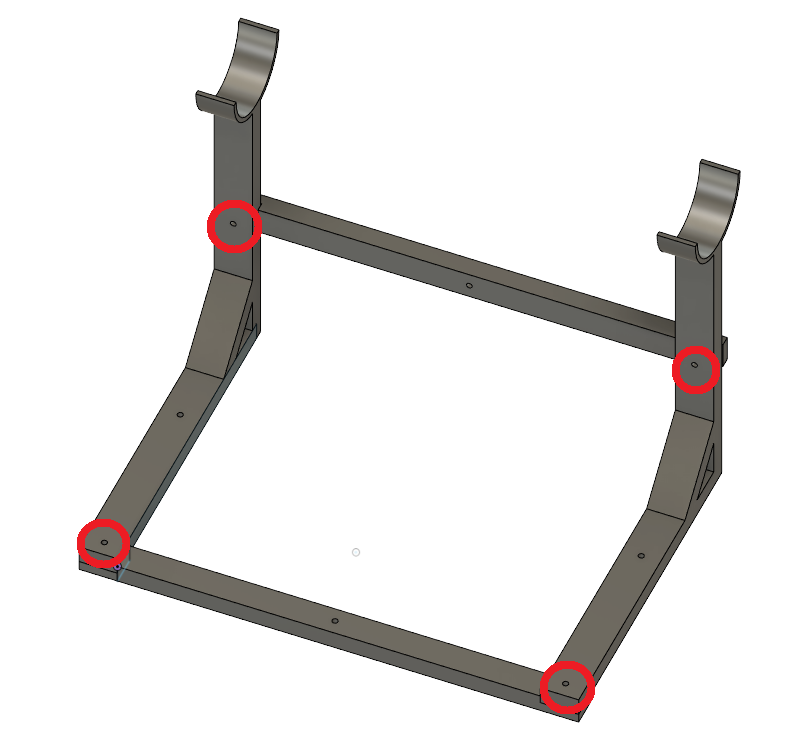
\includegraphics[width=12cm]{image/montage/boussole_solaire/2.png} 
\caption{Assemblage bases et longerons}
\end{figure}

Trois boulons de 3*30mm viennent se placer au endroits prevus, ces boulons permettent de regler la plaque de plexiglas pour qu'elle soit horizontal. La plaque de plexiglass est coupé dans du plexiglass de 3mm et les passage de boulon sont percer par une meche de 3mm. La plaque repose sur les trois boulons de 3*30mm.\\

\begin{figure}[H]
\centering
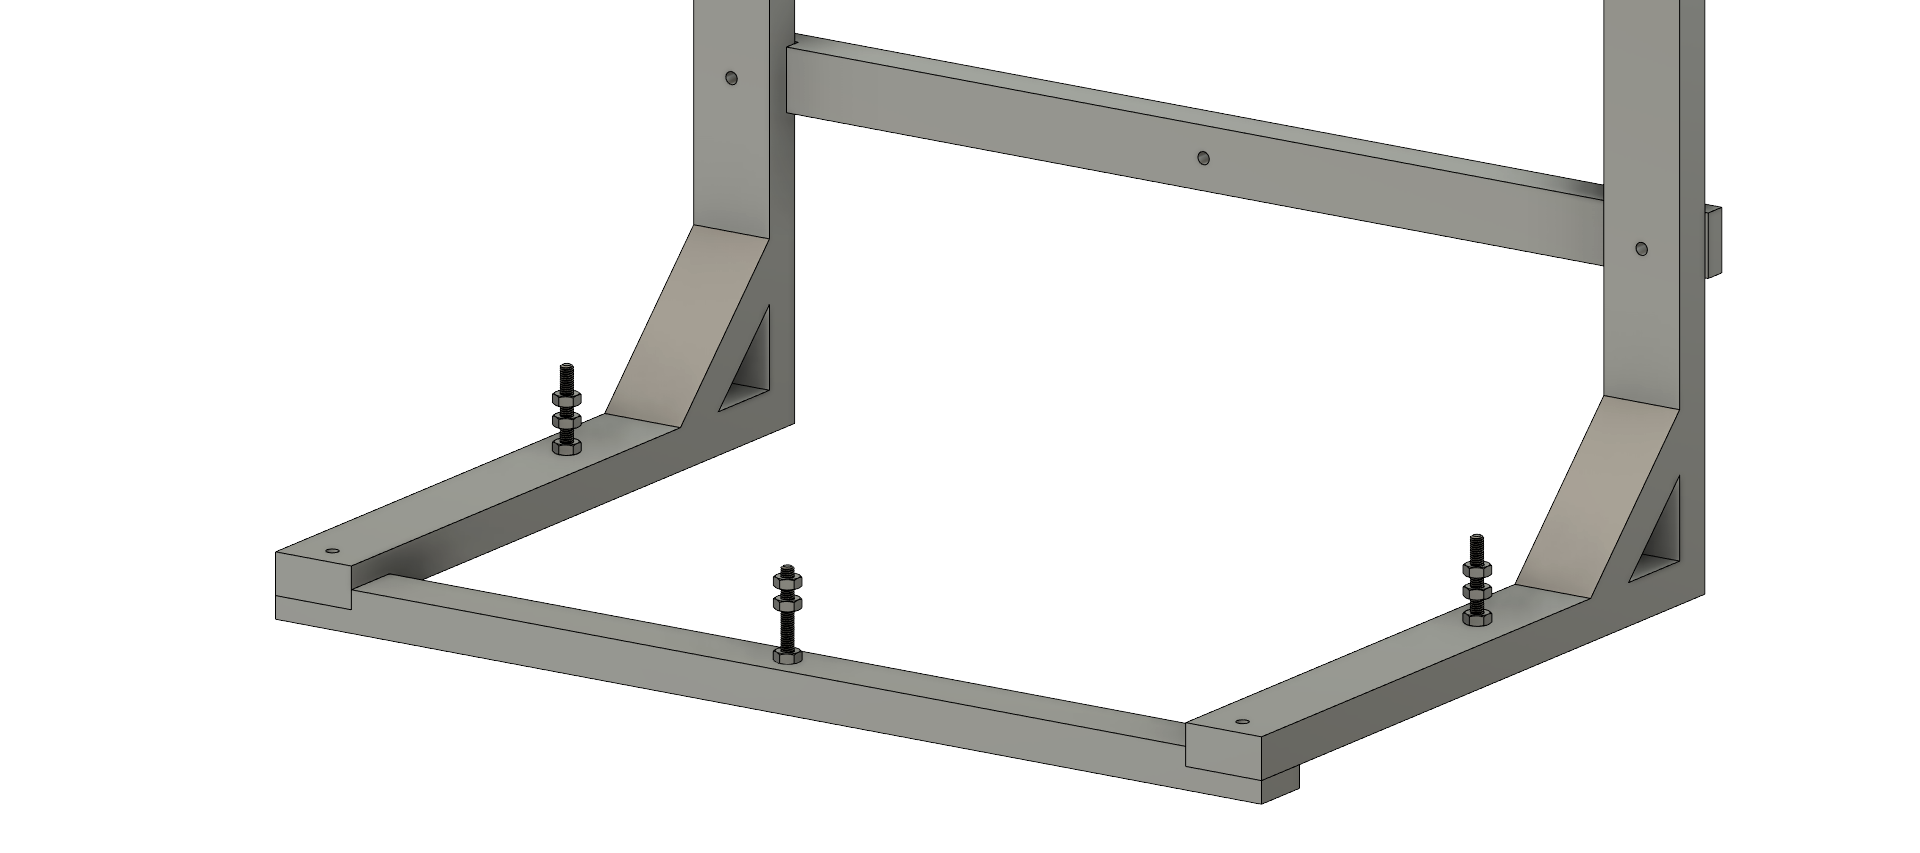
\includegraphics[width=12cm]{image/montage/boussole_solaire/6.png} 
\caption{cadran d'azimut}
\end{figure}

Le cadran d'azimut est imprimé sur du papier ordinaire puis plastifier pour resister aux intempérie, il est fixer sur la plaque de plexiglas grace à huit aimants qui permettent de faire coincider les bords pour assurer la paralelité avec la plaque de plexiglass et donc indirectement avec la barre transversale du cm121.\\

\begin{figure}[H]
\centering
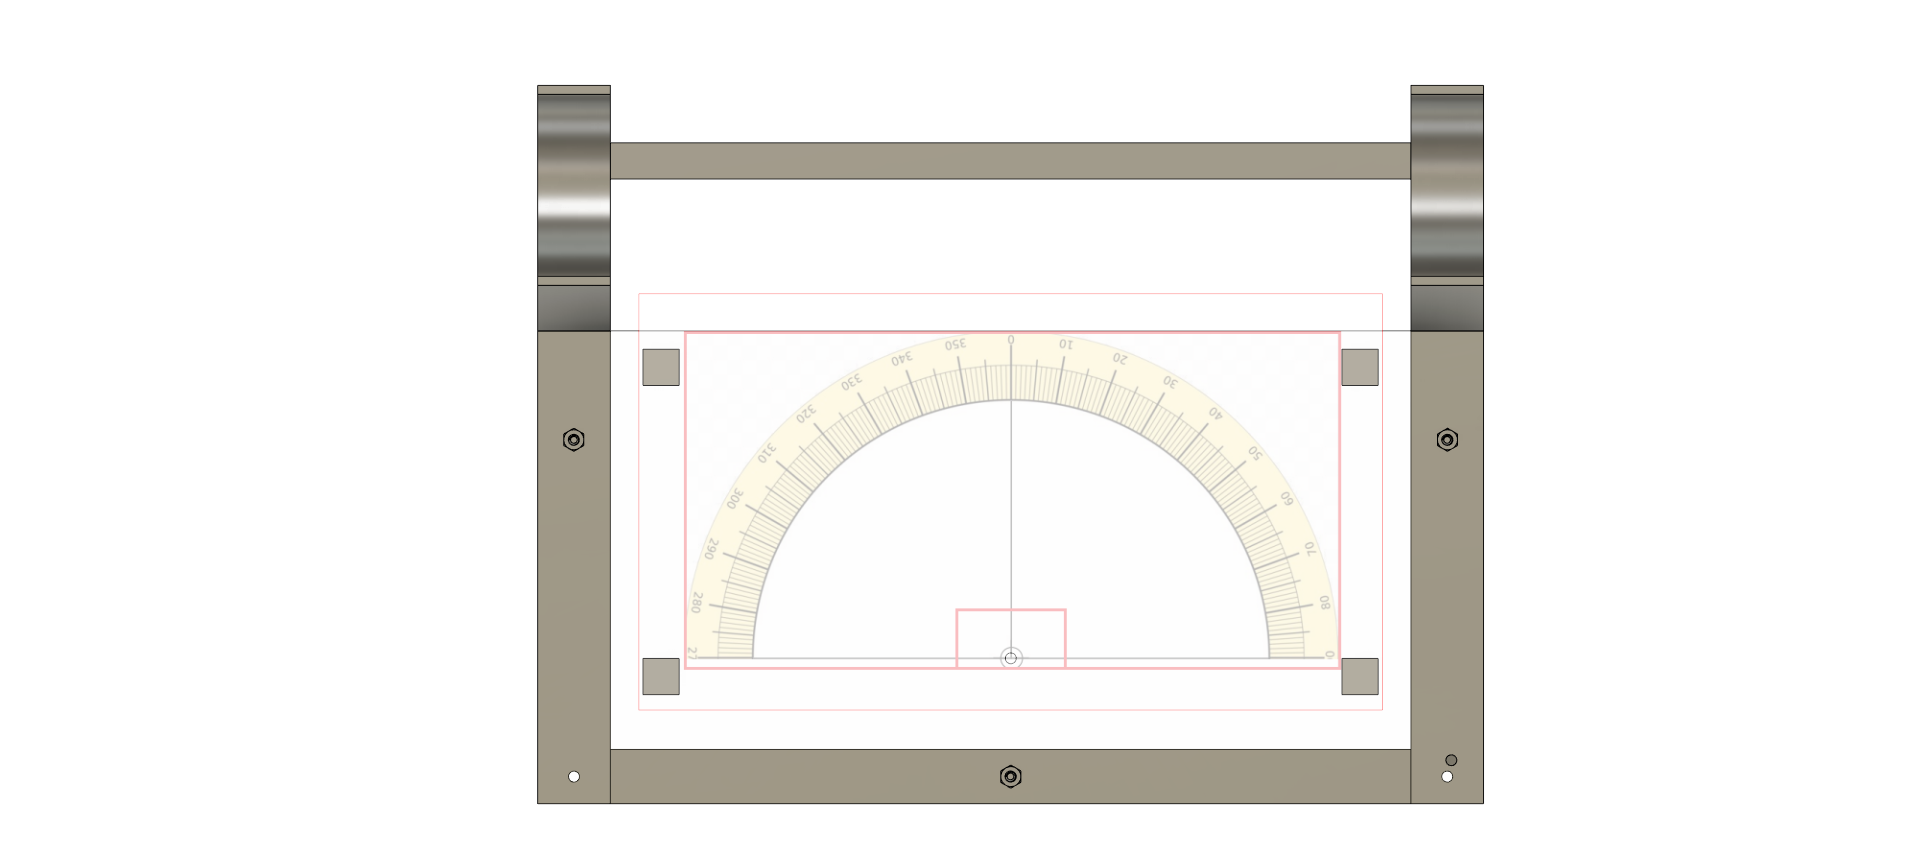
\includegraphics[width=12cm]{image/montage/boussole_solaire/5.png} 
\caption{cadran d'azimut}
\end{figure}


Viens ensuite la mise en place de la tige fileté de 3mm qui supporte le fil. Le fil passe dans l'intersection du cadran d'azimut et la plaque de plexiglass par un trou de 3mm, cela permet de reduire les effets du vents sur l'oscillation du fil.\\
Le cadran est par la suite fixer à la barre transversale à l'aide de colier rilsan, la plaque de plexiglas doit ensuite etre regler à l'horizontal, pour se faire un niveau de surface est utilisé est les ajustement se font par les trois boulons de 3*30mm.

\begin{figure}[H]
\centering
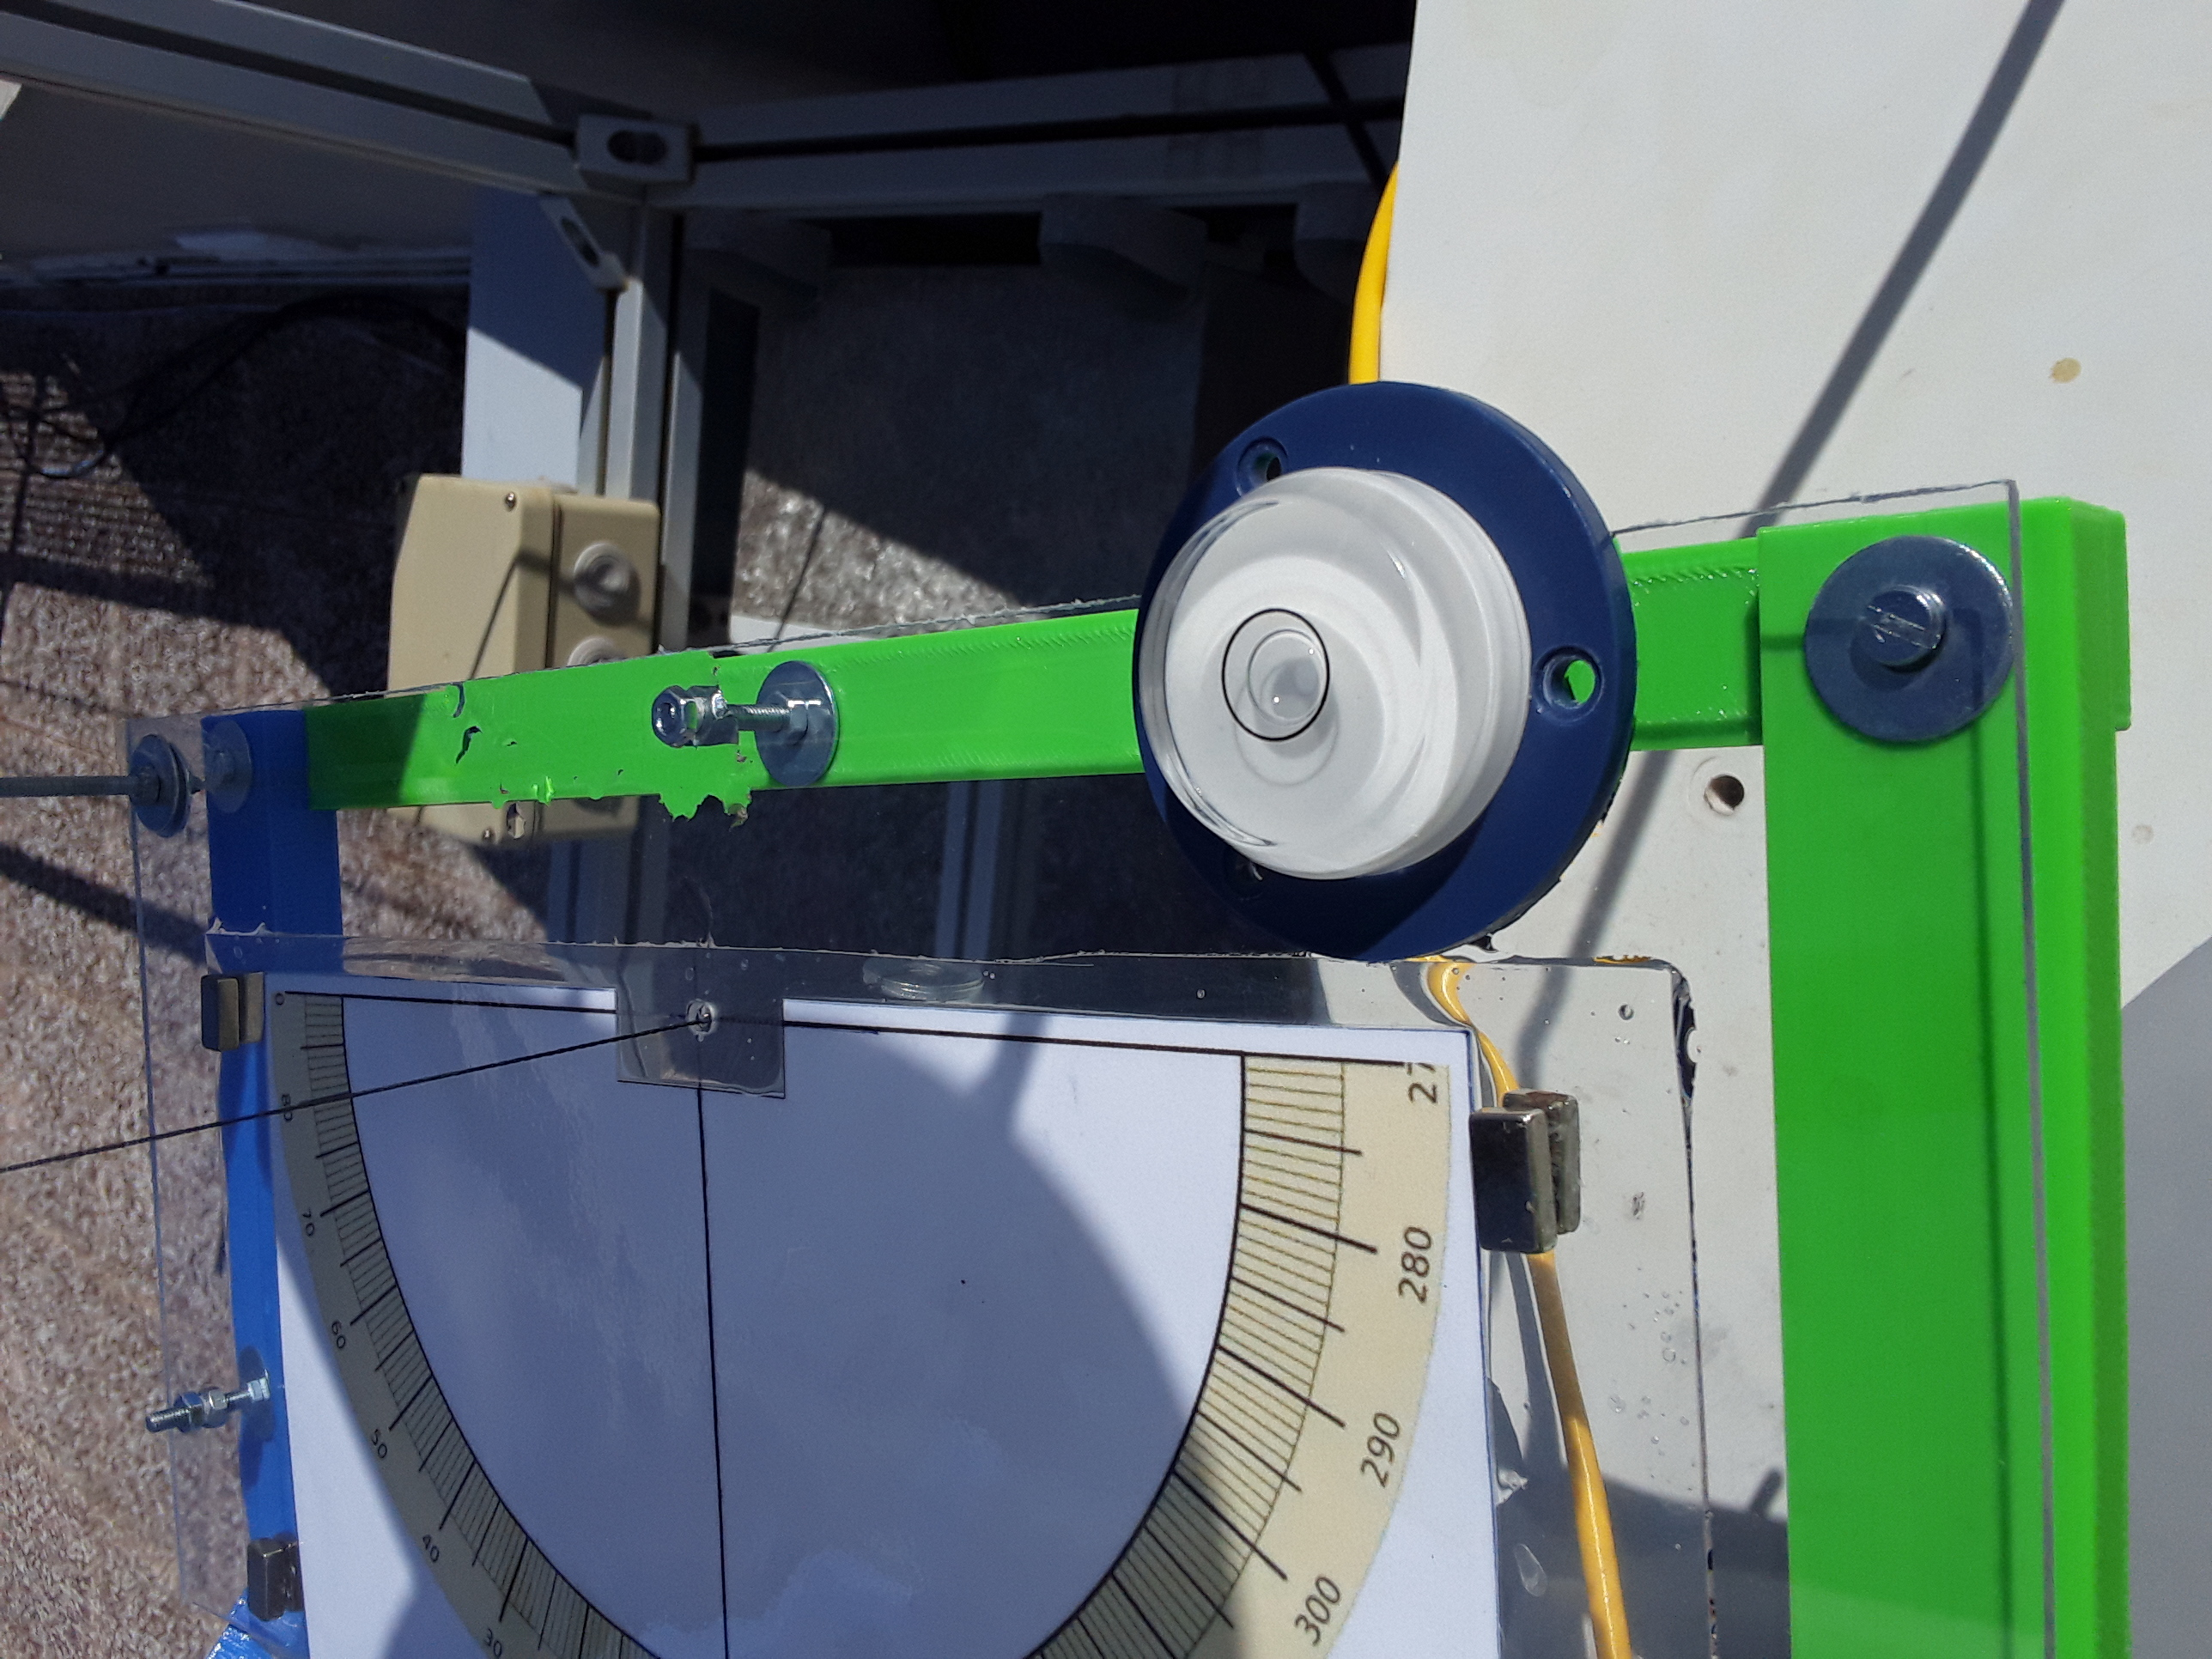
\includegraphics[width=12cm]{image/montage/boussole_solaire/7.jpg} 
\caption{cadran d'azimut}
\end{figure}

Nous devons maintenant connaitre l'azimut du soleil, la solution la plus simple est d'utiliser un site internet comme par exemple suncalc.org. L'azimut obtenu doit ensuite etre reporté sur le cadran, pour se faire il suffit de faire pivoter la base du cm121 sur son axe vertical. Le positionnement Nord-sud est effectué.\\
Cette méthode comporte quand meme des limites, elle ne marche que pour les jours ensoleillé et la présence de masque cache à certain moment de la journée le soleil ce qui empeche le positionnement nord-sud. 
 
\section{Programmation}

\subsection{Calendrier du Cm121}

Le calendrier de maintenance du CM121 comporte deux informations, l'heure du midi solaire et la position de la barre coulissante.

La position de la barre coulissante est calculé en fonction de la déclinaison du soleil, par l'expression : 

\begin{flalign*}
&L = 297 tan (\delta)&&\\
\end{flalign*}
Avec :\\
L : la position de la barre coulissante\\
$\delta$ : la déclinaison du soleil\\
~~\\

Nous pouvons retrouver cette equation en appliquant pythagore sur la figure suivante:

\begin{figure}[H]
\centering
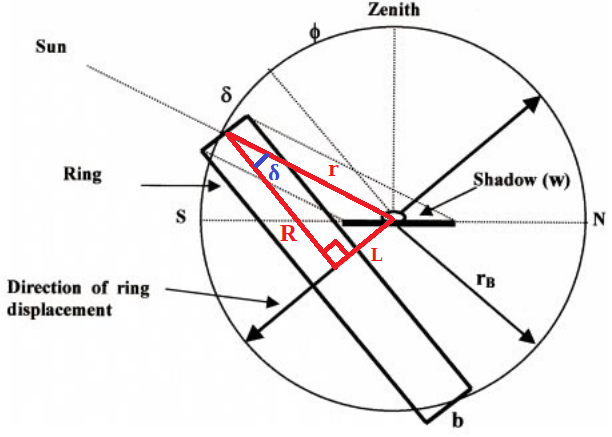
\includegraphics[width=8cm]{image/calendrier/1.PNG}  
\end{figure}

\begin{flalign*}
&R = 297~mm&&\\
&tan(\delta) = \frac{L}{R}&&\\
&L = R~tan(\delta)&&\\
&L = 297tan(\delta)&&\\
\end{flalign*}

Les calendriers sont calculer par la fonction principale calendrier.py (voir annexe), pour faciliter l'éxécution du programme, celui-ci s'éxécute via un terminal par la ligne de commande :
\begin{flalign*}
&\$python~ calendrier.py ~année 
\end{flalign*}

Le programme retourne alors trois calendrier, un calendrier au format csv, un calendrier au format xlsx et un calendrier ics. Le calendrier csv est obtenue par du texte brut ce qui siginifie qu'il fonctionne avec tout les logiciels de traintement de texte, mais ne permet pas la mise en forme. Le calendrier xlsx permet d'intégrer la mise en forme au calendrier, nous obtenons ainsi des codes couleurs, en vert les jours fériés, en bleu les weekends et en rouge les maintenances minimum à effectuer sur le cm121. Le calendrier ics permet d'avoir les positions du cm121 au format iCalendar ce qui permet entre autre d'avoir le midi-solaire et la position de la barre coulissante via son smartphone.

\begin{figure}[H]
\centering
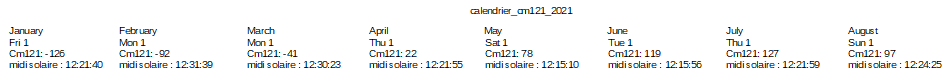
\includegraphics[width=16cm]{image/calendrier/3.PNG} 
\caption{calendrier au format csv}  
\end{figure}

\begin{figure}[H]
\centering
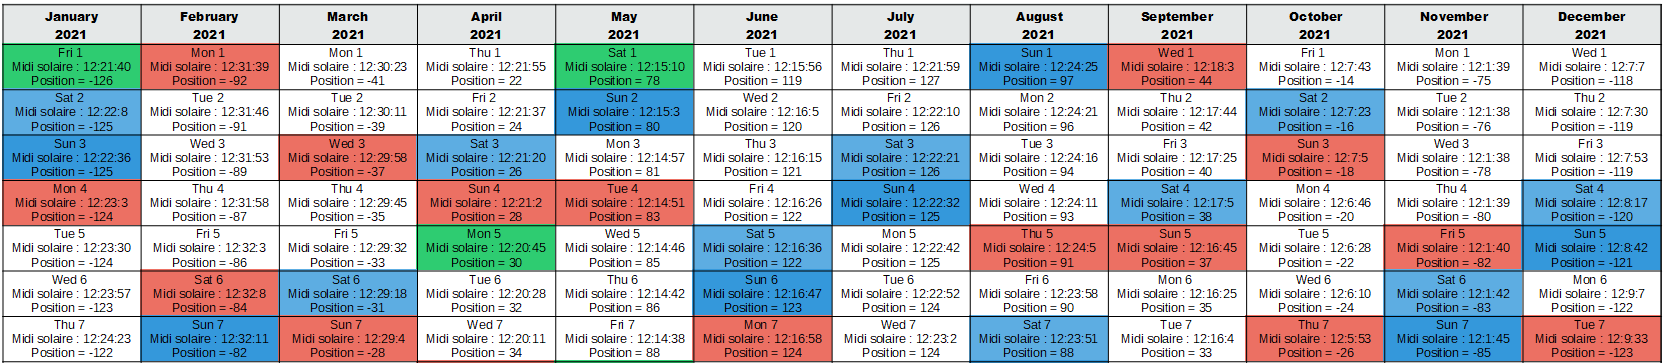
\includegraphics[width=16cm]{image/calendrier/2.PNG} 
\caption{calendrier au format xlsx}  
\end{figure}

\begin{figure}[H]
\centering
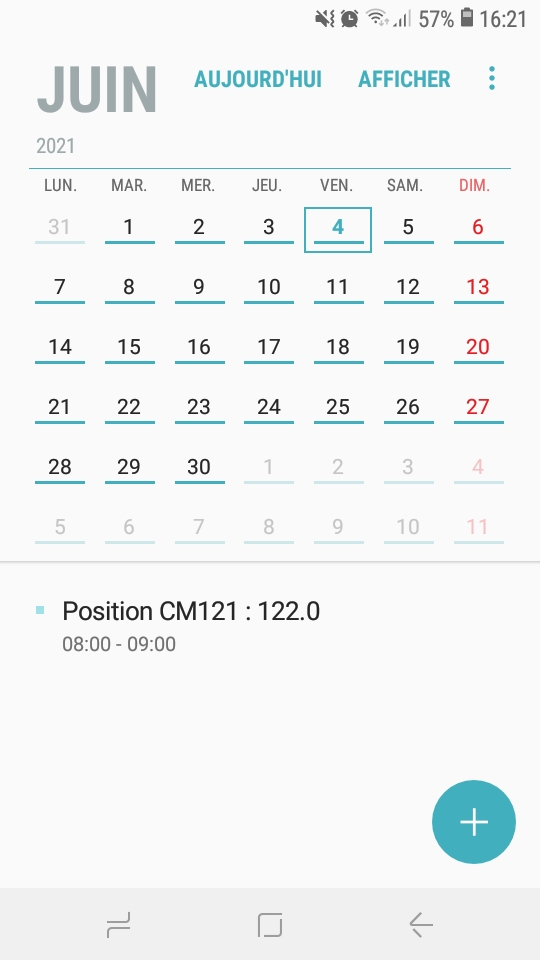
\includegraphics[width=5cm]{image/calendrier/4.jpg} 
\caption{calendrier au format ics}  
\end{figure}

\subsection{Analyse statistique}

J'ai du lors du stage dévelloper des programmes en python permettant d'effectuer l'analyse statistique d'un jeu de donnée. Pour ce faire mes programmes fonctionne avec des dataframes, j'ai porté mon choix vers les dataframes car elles sont facile à manipuler. 

\subsubsection{Suppression des données non utilisés, non acquis et abérantes}

Le fichier de mesure comporte généralement des données non acquis pouvant bloquer l'éxécution de certain programme, mais aussi les données pour la nuit qui sont inintéressante dans le cas de létude du DHI ou du GHI. La fonction nettoyage.py (voir annexe) permet d'enlever ces valeurs. 

\subsubsection{Calcul des facteurs de correction}

Les données du cm121 doit etre corrigés car l'arc d'ombrage masque une partie du diffus. L'expression permettant de calculer le facteur de correction donné dans la datasheet se base sur les travaux de Drummond, cette correction fait l'hypothèse que le ciel est isotropique ce qui donne une correction des mesures purement géométrique (voir annexe).\\

Les mesures du CM121 sont corrigées par la fonction correction\_kippzonen.py (voir annexe), cette focntion calcul le facteur de correction en se basant sur l'heure ou la mesure a été prise et l'applique aux mesures du cm121.

\subsubsection{Etalonnage}

Lors de l'étallonnage les mesures subissent une régression linéaire par rapport à des mesures de références, nous obtenons alors une droite d'équation $y = ax + b$ que nous voulons ramener pour obtenir une droite d'équation $y = x$.\\

La fonction regression\_lineaire.py permet d'effectuer l'étalonnage (voir annexe). Outre l'étallonage la fonction regression\_lineaire.py éffectue aussi l'analyse statistique. L'analyse statistique permet d'obtenir sur le graphique le coefficient de détermination $R^2$, la variance, l'erreur quadratique moyenne et  l'erreur absolue moyenne.\\

Le coefficient de détermination $R^2$ est un indicateur qui permet de juger la qualité d’une régression linéaire. Si le $R^2$ vaut 1, cela signifie que l’équation de la droite de régression est capable de déterminer 100 \% de la distribution des points. Cela signifie alors que le modèle mathématique utilisé, ainsi que les paramètres a et b calculés sont ceux qui déterminent la distribution des points.\\
~~\\
La variance est une mesure de la dispersion des valeurs d'un échantillon.
~~\\
L'erreur quadratique moyenne (RMSE) fournit une indication par rapport à la dispersion ou la variabilité de la qualité de la prédiction, il est souvent relié à la variance car les valeurs de RMSE sont difficiles à interpréter parce que l’on est pas en mesure de dire si on a une variance faible ou forte, l'erreur quadratique moyenne donne plus de poids aux erreurs élevés.
~\\ 

\begin{figure}[H]
\centering
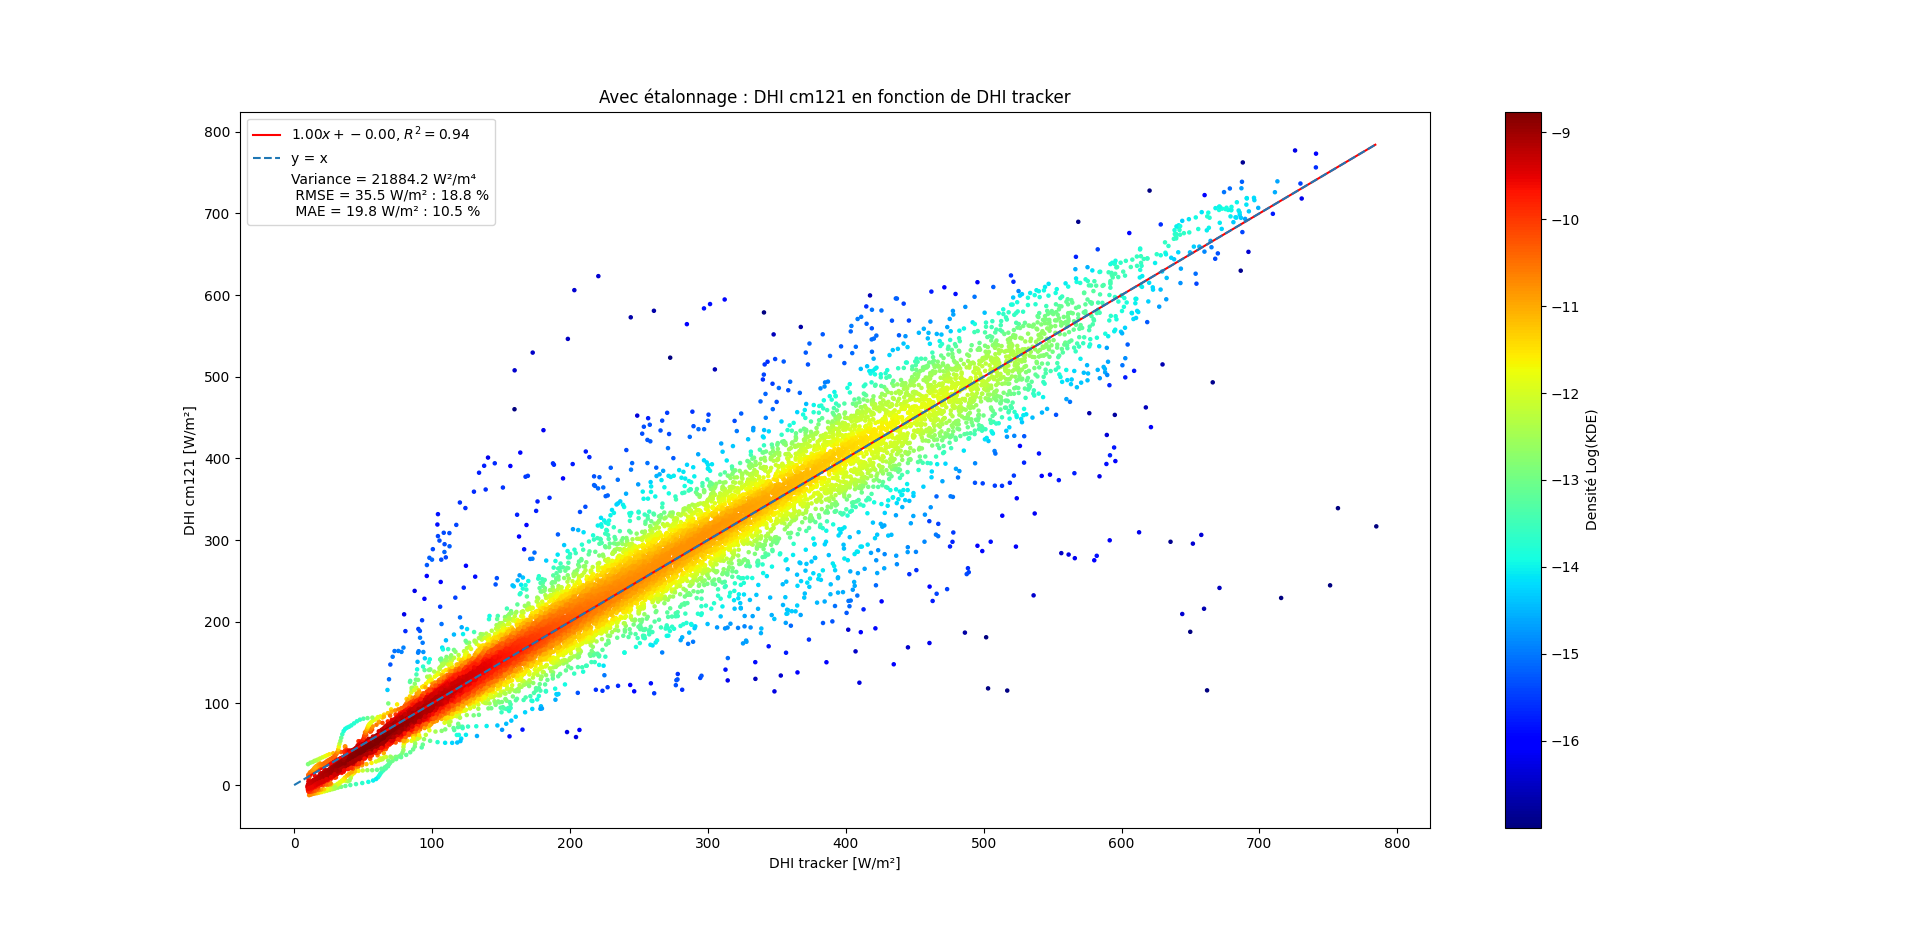
\includegraphics[width=15cm]{image/etallonnage/1.png} 
\caption{régression linéaire}  
\end{figure}

\subsection{Représentation graphique de l'erreur relative}

La fonction erreur\_relative.py donne la représentation de l'erreur relative en fonctions de l'azimut et de l'élévation du soleil permet de mettre en lumière des journées particulières comme par exemple le dysfonctionnement de l'acquisition des mesures, mais aussi la presence de masque ou de reflet impactant le pyranomètre. Les erreurs aberantes qui sont identifer grace à cette méthode peuvent donc etre supprimé.\\
 
\begin{figure}[H]
\centering
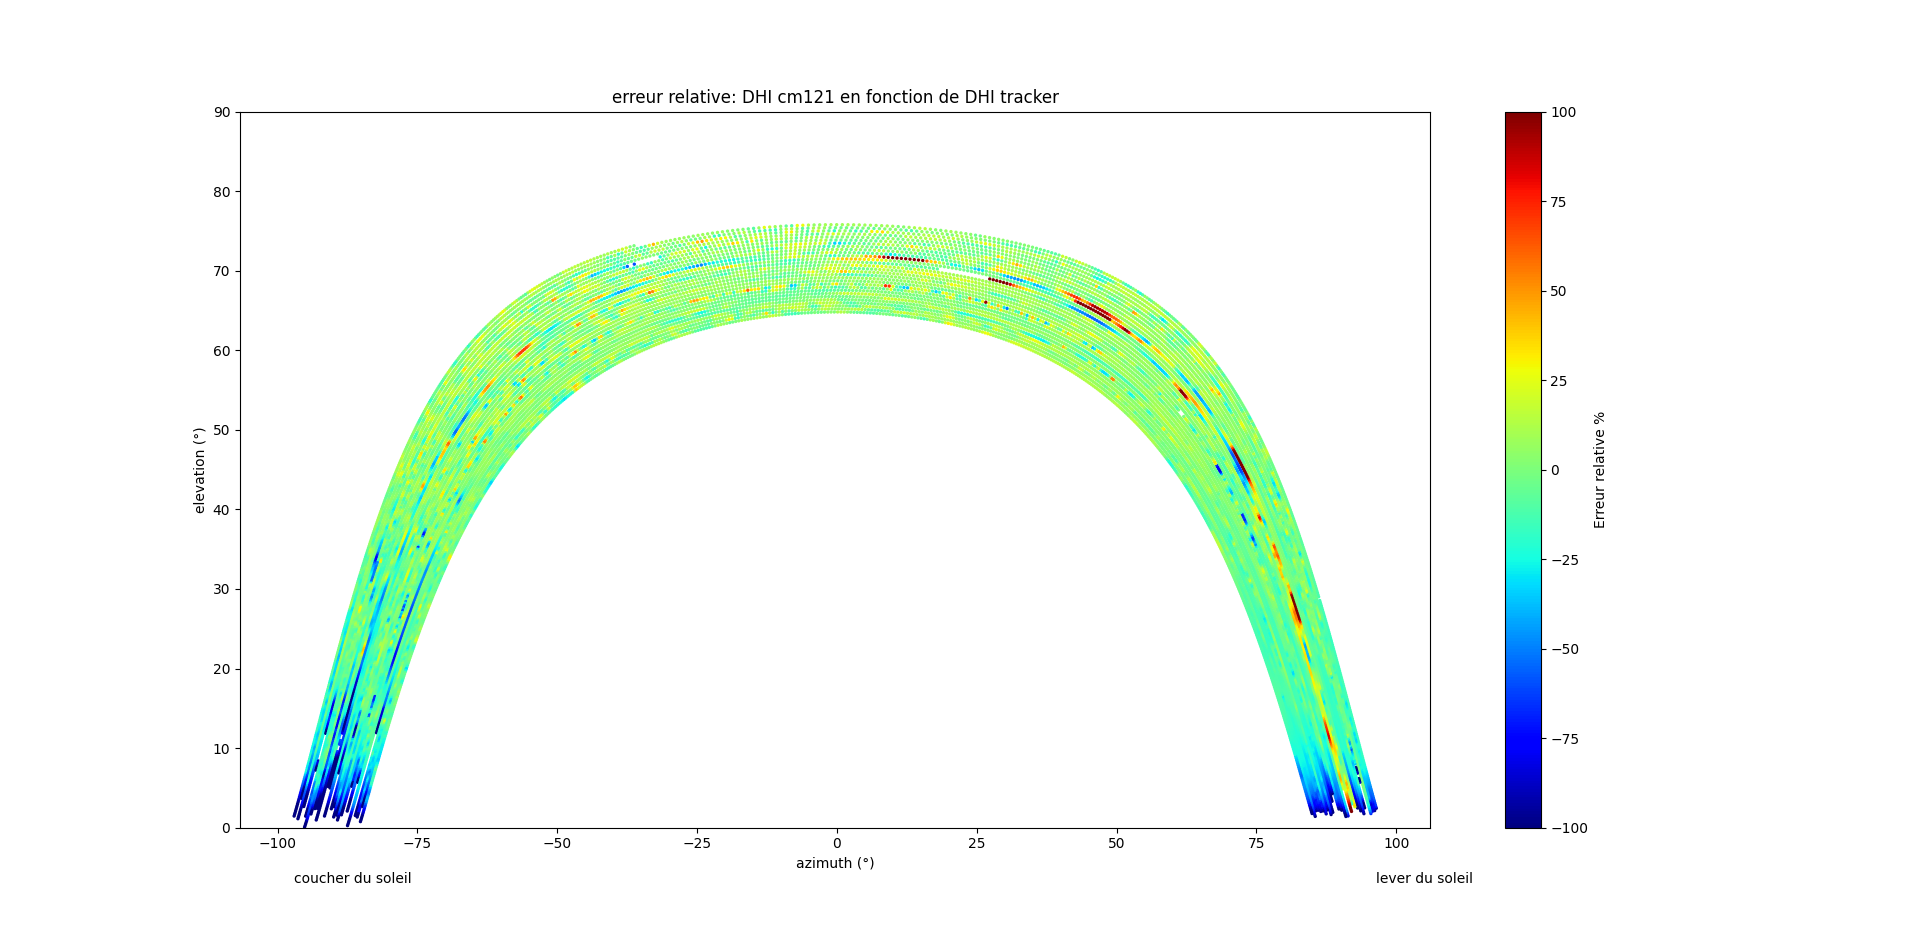
\includegraphics[width=15cm]{image/erreur_relative/1.png} 
\caption{régression linéaire}  
\end{figure}

\subsubsection{Histogramme}

La fonction histogramme.py donne la représentation graphique de la répartition dune variable, dans notre cas la fonction donne la répartition du rayonnement diffus et de l'erreur relative.\\

\begin{figure}[H]
\centering
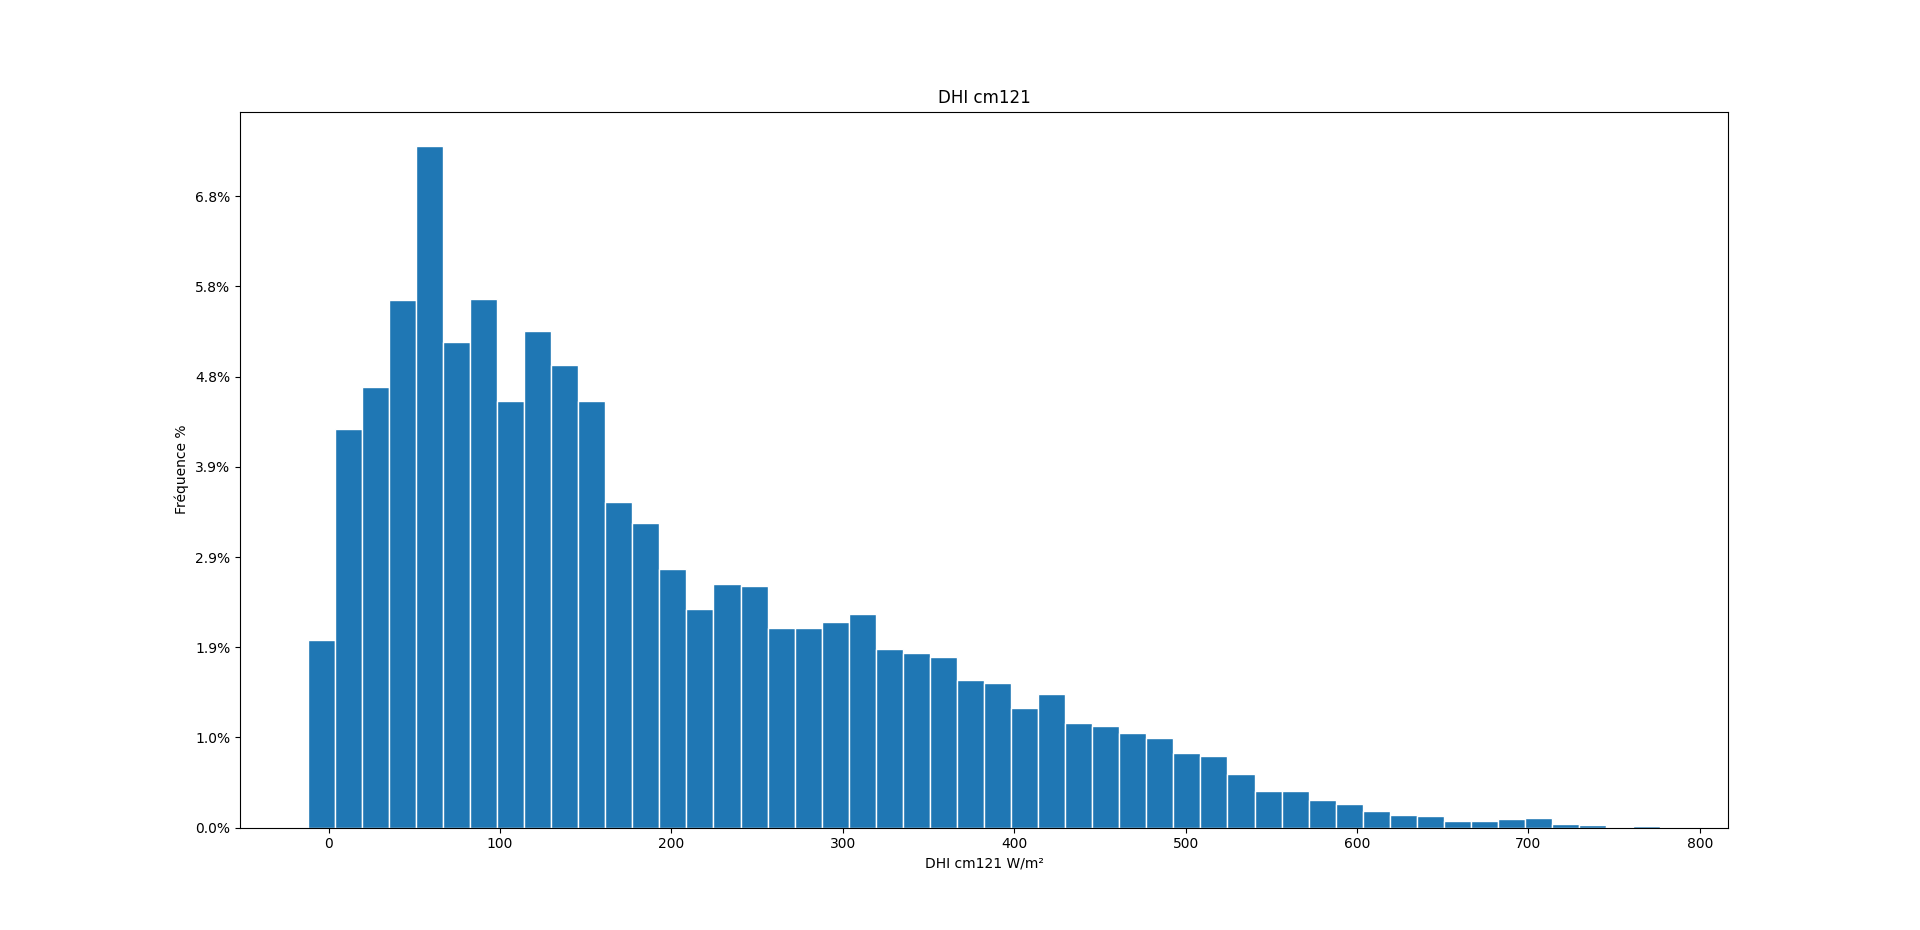
\includegraphics[width=15cm]{image/histogramme/1.png} 
\caption{régression linéaire}  
\end{figure}

\begin{figure}[H]
\centering
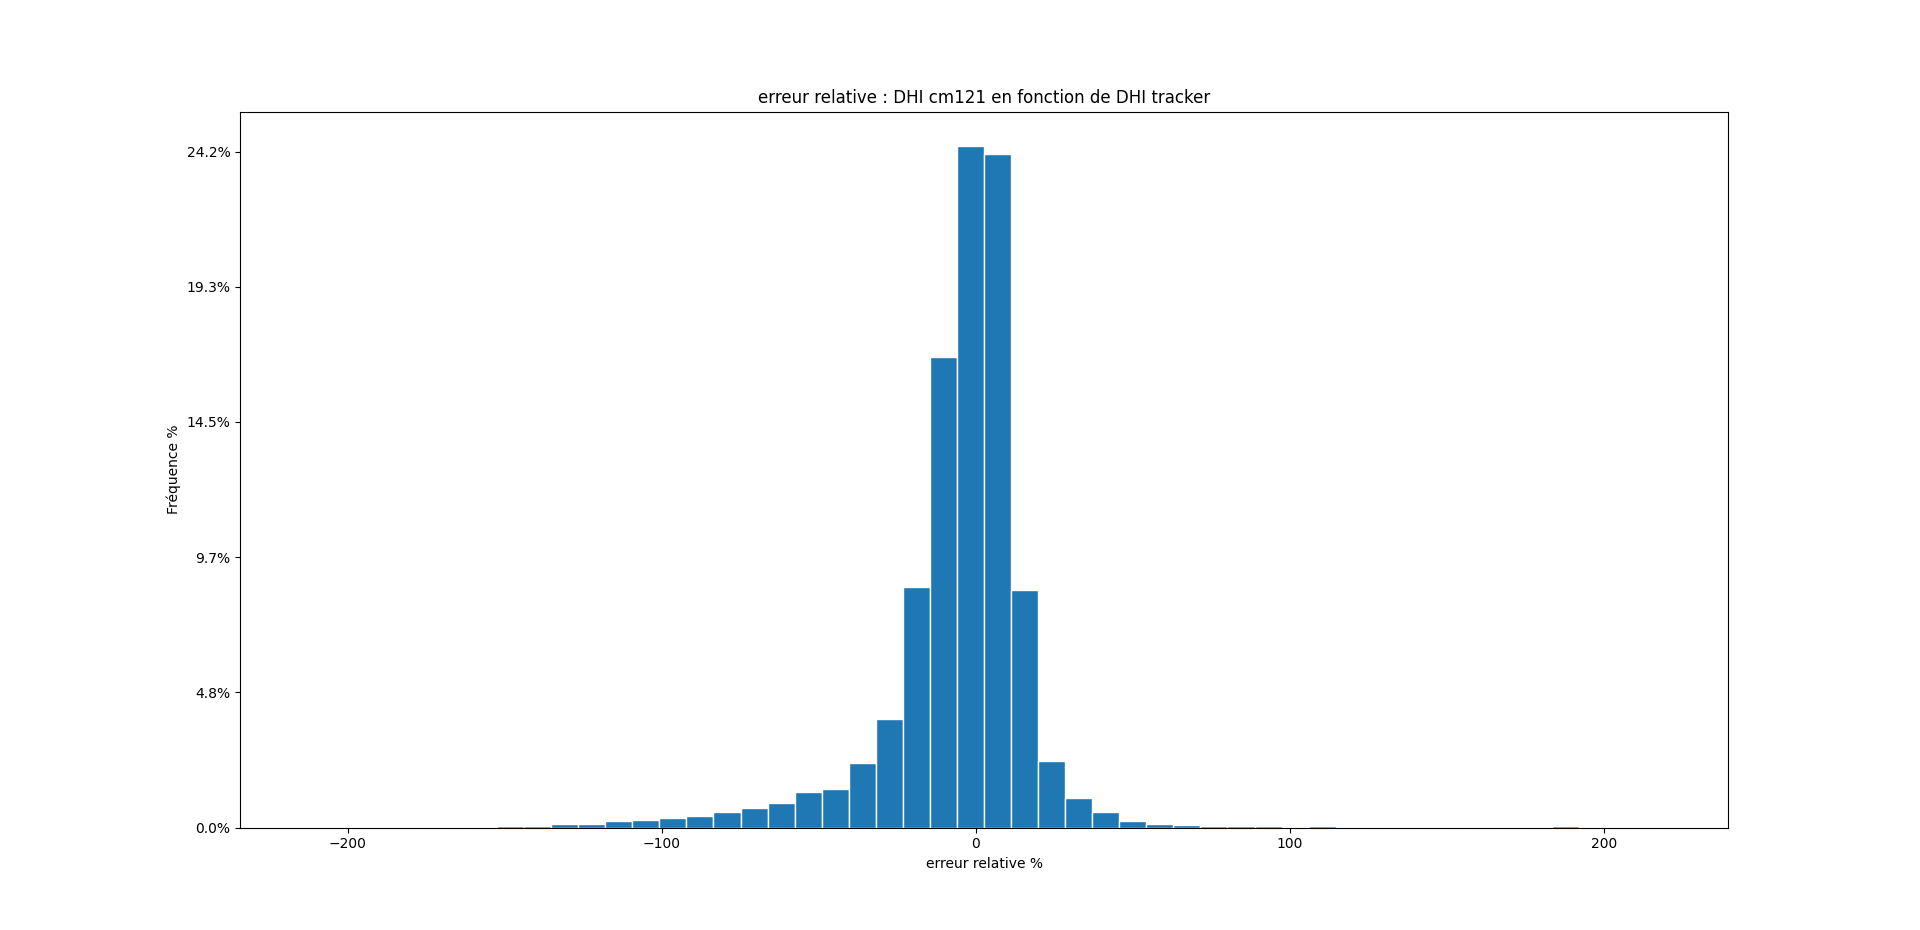
\includegraphics[width=15cm]{image/histogramme/2.png}  
\caption{régression linéaire}  
\end{figure}

\subsubsection{Selection des mesures entre deux intervalles}

Deux fonctions ont été creer pour selectionner les mesures entre une periode donnée, la première permet d'avoir les mesures entre deux dates et la derniere permet d'avoir les mesure pour une tranche horaire spécifié. Ces deux foncions permettent de savoir qu'elle dispositif donne de meilleur mesure que ce soit pour le matin ou l'après-midi, et pendant les saison été hiver.

\subsubsection{éxécution de l'analyse statistique}

Pour faciliter l'utilisation du programme celui-ci s'éxécute via un terminal, pour ce faire l'utilisateur doit juste renseigner le nom de son fichier de mesure, choisir les valeurs tests et les valeurs pour la référence. Si l'utilisateur le souhaite il est aussi en mesure de renseigner la periode sur laquel il souhaite l'analyse statistique.

\subsubsection{Etallonage du cm121 avec le spn1}

Le CM121 et le spn1 utilise tous deux un arc pour masquer le rayonnement direct du soleil, cet arc donne un angle de vue de 10.8° pour le cm121 et le spn1 comparer à un angle de vue de 4.5° pour le masque du tracker.

\subsubsection{Impact de la ventillation sur les mesures du cm121}

Les mesures avec la ventillation opérationnelle ont été acquise entre le 21 avril 2021 et le 31 mai 2021, nous devons donc comparer les mesures avec ventillation et sans ventillation sur la meme periode de 41 jours, les mesures entre  entre le 21 avril 2021 et le 31 mai 2021 sont comparer aux mesures entre le 11 mars et le 20 avril.

\begin{figure}[H]
\centering
\includegraphics[width=15cm]{image/impact_ventillation/avril_mai_2021/regression_avec_étalonnage_DHI cm121vsDHI tracker.png} 
\caption{régression linéaire période avec ventillation}  
\end{figure}

\begin{figure}[H]
\centering
\includegraphics[width=15cm]{image/impact_ventillation/archive_2021-03-11_2021-04-20/regression_avec_étalonnage_DHI cm121vsDHI tracker.png}  
\caption{régression linéaire période sans ventillation}  
\end{figure}

\begin{figure}[H]
\centering
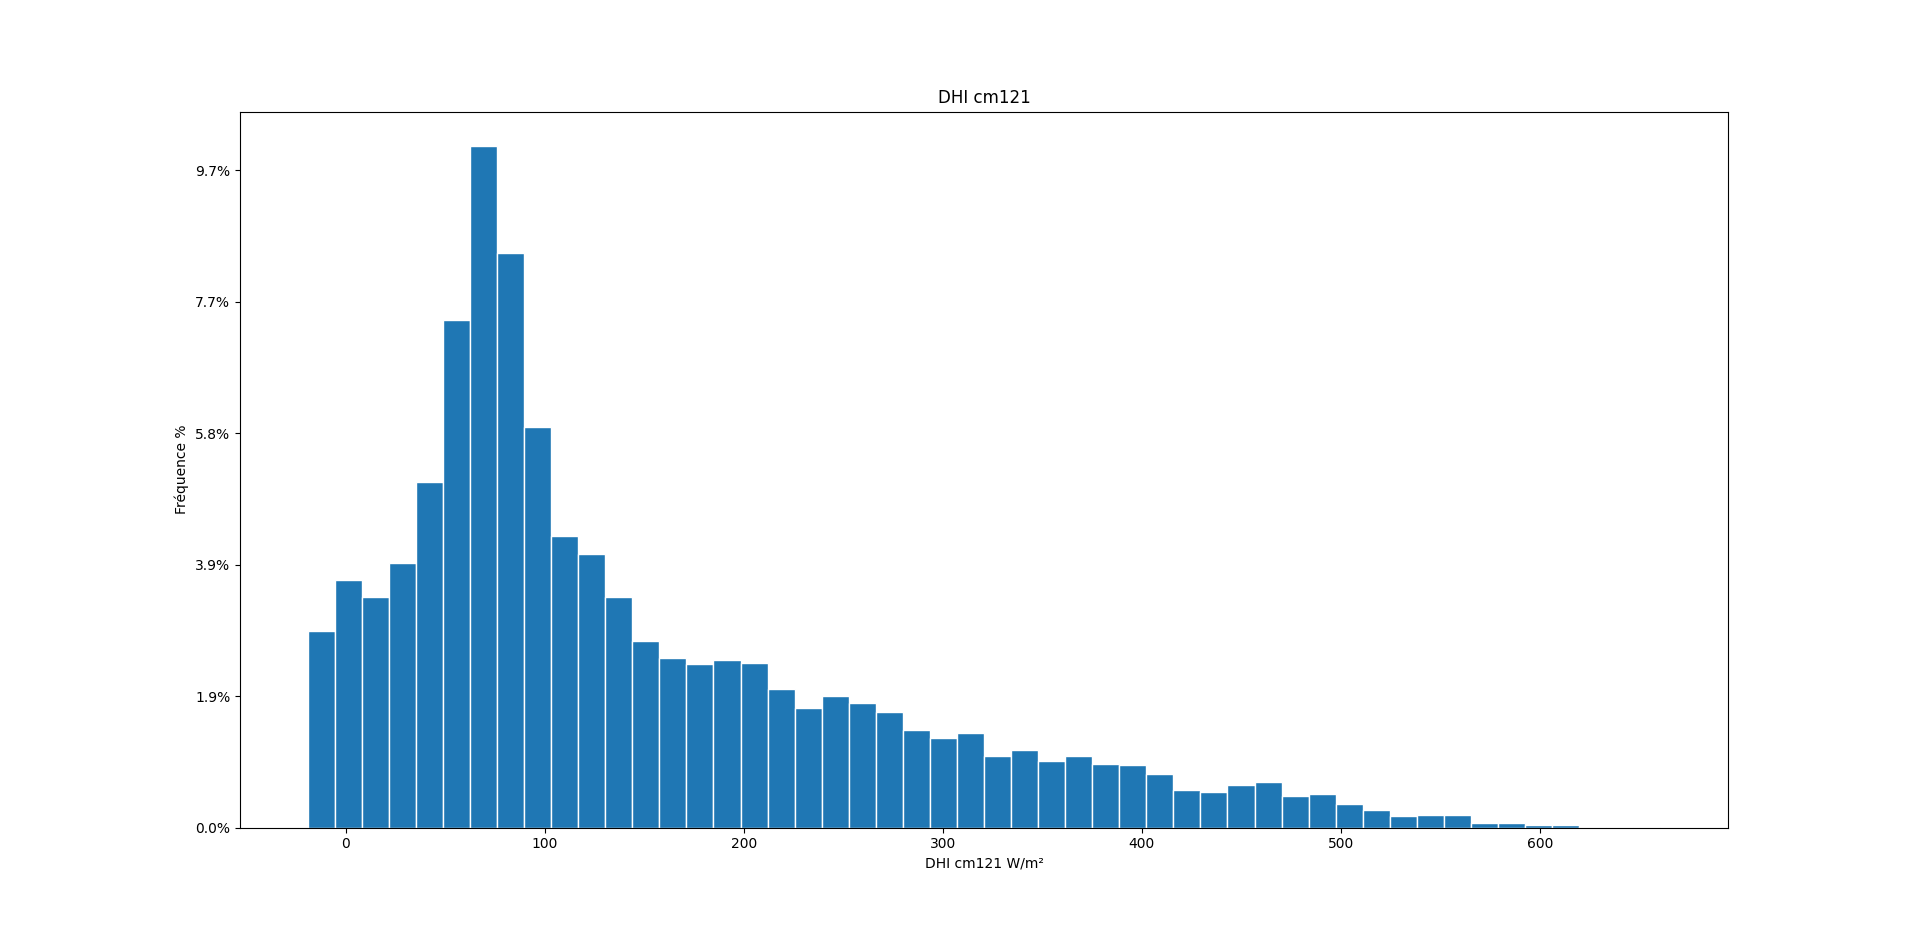
\includegraphics[width=15cm]{image/impact_ventillation/avril_mai_2021/histogramme_3.png}  
\caption{répartition du DHI avec ventillation}  
\end{figure}

\begin{figure}[H]
\centering
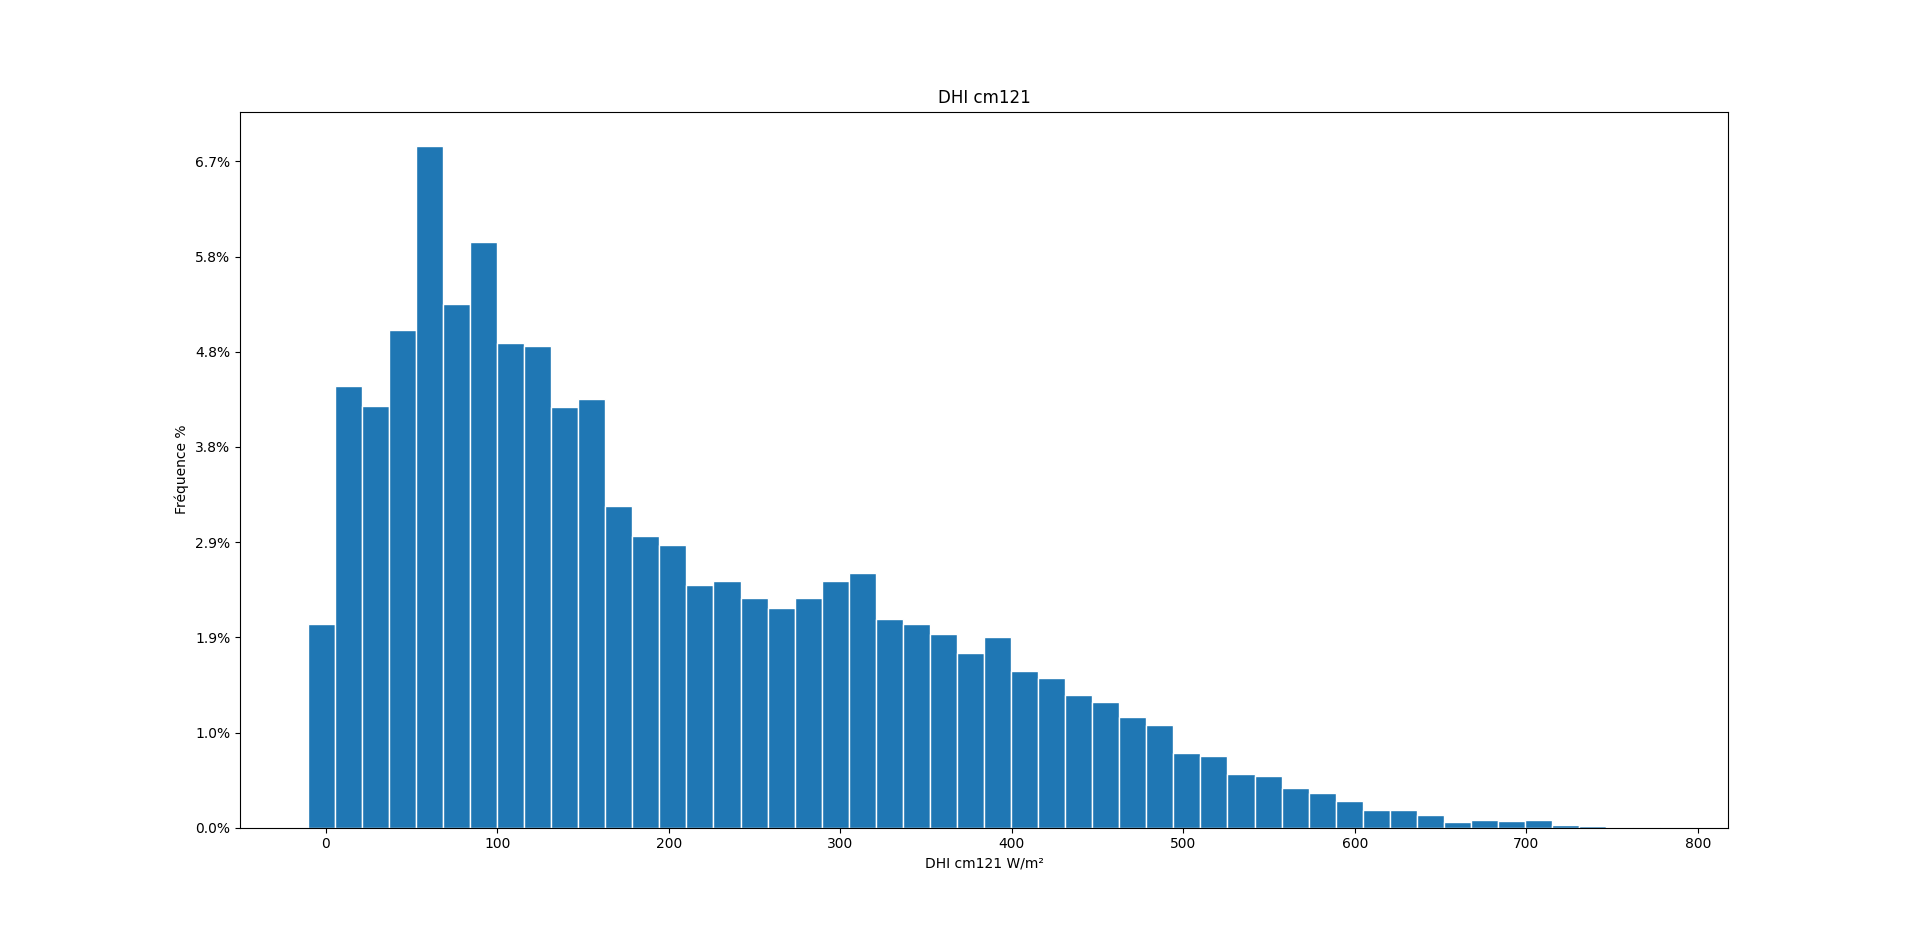
\includegraphics[width=15cm]{image/impact_ventillation/archive_2021-03-11_2021-04-20/histogramme_3.png} 
\caption{répartition du DHI sans ventillation}  
\end{figure}

Nous obtenons avec la mise en place de la ventillation un RMSE et un MAE plus élevé, dire que l'ajout de la ventillation entraine une augmentation de la dispersion des mesures semble fausse. Les histogramme nous montrent que pour les deux périodes la répartition du dhi est similaire. J'en conclue que nous ne pouvons pas voir un réel impact de la ventillation sur une période aussi petite.





\end{flushleft}





%\begin{figure}[H]
%\centering
%\includegraphics[width=25cm]{} 

%\end{figure}

\end{document}